% ****** Start of file aipsamp.tex ******
%
%   This file is part of the AIP files in the AIP distribution for REVTeX 4.
%   Version 4.1 of REVTeX, October 2009
%
%   Copyright (c) 2009 American Institute of Physics.

% Use this file as a source of example code for your aip document.
% Use the file aiptemplate.tex as a template for your document.
\documentclass[%
 aip,
 jmp,%
 amsmath,amssymb,
%preprint,%
 reprint,%
 floatfix,
%author-year,%
%author-numerical,%
]{revtex4-1}
\usepackage{graphicx}% Include figure files
\usepackage{grffile}
\usepackage{dcolumn}% Align table columns on decimal point
\usepackage{bm}% bold math
%\usepackage[mathlines]{lineno}% Enable numbering of text and display math
%\linenumbers\relax % Commence numbering lines
\usepackage{multirow}
\usepackage{color} % for the notes
\usepackage{etex}
\reserveinserts{58}
%\usepackage{morefloats}
\usepackage{hyperref}
\usepackage{xcolor}
\usepackage{amsmath}
\hypersetup{
        colorlinks,
        linkcolor={red!50!black},
        citecolor={blue!50!black},
        urlcolor={blue!80!black}
}
%\usepackage{placeins}
\usepackage{xr}
\externaldocument{paper}
\usepackage[section] {placeins}

\begin{document}

\preprint{XXXXX (preprint)}

%\title[Evolution of interaction networks]{On the evolution of interaction networks: primitive typology of vertex, prominence of measures and activity statistics}% Force line breaks with \\
%\title[Evolution of interaction networks]{On the evolution of interaction networks: a primitive typology of vertex}% Force line breaks with \\
\title[Stability of interaction networks, SUPPORTING INFORMATION]{Stability in human interaction networks: primitive typology of vertex, prominence of measures and time activity statistics, SUPPORTING INFORMATION}% Force line breaks with \\

\author{Renato Fabbri}%
 \homepage{http://ifsc.usp.br/~fabbri/}
 \email{fabbri@usp.br}
  \affiliation{ 
S\~ao Carlos Institute of Physics, University of S\~ao Paulo (IFSC/USP)%\\This line break forced with \textbackslash\textbackslash
}

\author{Vilson V. da Silva Jr.}
  \homepage{http://automata.cc/}
  \email{vilson@void.cc}
  \altaffiliation[Also at ]{IFSC-USP}%Lines break automatically or can be forced with \\

\author{Ricardo Fabbri}
  \homepage{http://www.lems.brown.edu/~rfabbri/}
  \email{rfabbri@iprj.uerj.br}
 \altaffiliation{
Instituto Polit\'ecnico, Universidade Estadual do Rio de Janeiro (IPRJ)
}%Lines break automatically or can be forced with \\

\author{Deborah C. Antunes}
  \homepage{http://lattes.cnpq.br/1065956470701739}
  \email{deborahantunes@gmail.com}
  \altaffiliation{
Curso de Psicologia, Universidade Federal do Cer\'a (UFC)
}%Lines break automatically or can be forced with \\

\author{Marilia M. Pisani}
  \homepage{http://lattes.cnpq.br/6738980149860322}
  \email{marilia.m.pisani@gmail.com}
 \altaffiliation{
Centro de Ci\^encias Naturais e Humanas, Universidade Federal do ABC (CCNH/UFABC)
}%Lines break automatically or can be forced with \\

%
%%\author{Luciano da Fontoura Costa}
%%  \homepage{http://cyvision.ifsc.usp.br/~luciano/}
%%  \email{ldfcosta@gmail.com}
%  \altaffiliation[Also at ]{IFSC-USP}%Lines break automatically or can be forced with \\

%\author{Osvaldo N. Oliveira Jr.}
%  \homepage{www.polimeros.ifsc.usp.br/professors/professor.php?id=4}
%  \email{chu@ifsc.usp.br}
% \altaffiliation[Also at ]{IFSC-USP}%Lines break automatically or can be forced with \\


\date{\today}% It is always \today, today,
             %  but any date may be explicitly specified

\begin{abstract}
 This is the supporting information of the article that reports interaction networks stability by means of three quantitative criteria: activity distribution in time and among participants; a sound classification of vertices in peripheral, intermediary and hub sectors; the combination of basic measures into principal components with greater variance. 
\end{abstract}

\pacs{89.75.Fb,05.65.+b,89.65.-s}% PACS, the Physics and Astronomy
\keywords{complex networks, social network analysis, pattern recognition, statistics, anthropological physics}
\maketitle

These results were produced with the Gmane public domain data and an open python package designed for attaining
these, and related, results. The interested reader should follow Appendix~\ref{scripts} to access both data and rotines.
Inline are results for 4 emails lists: LAD, LAU, MET and CPP, as described in Section~\ref{sec:data}.
Similar results can be reproduced for any number of (Gmane) email lists.
To avoid repeating text of each table for each list, the text is given inline.

\section{Time tables in different scales}\label{sec:time}
Theory presented in Section~\ref{sec:mtime} and results exposed in Section~\ref{constDisc} of the paper~\cite{tpaper}.
\subsection{Time circular measures}
The rescaled circular mean $\theta_\mu'$, the standard deviation $S(z)$, the variance $Var(z)$, the circular dispersion $\delta(z)$ and the relation of maximum and minimum incidence at each time unit $\frac{max(incidence}{min(incidence}$. Also, $ \mu_{\frac{max(incidence')}{min(incidence')}} $ and $ \sigma_{\frac{max(incidence')}{min(incidence')} }$ are given for 1000 uniform distribution simulations within the same number of bins and with the same number of samples. Section~\ref{sec:mtime} describes the theoretical background of directional (or circular) statistics.
\begin{table*}[!h]
	\caption{LAU circular measures}
\begin{center}
    \begin{tabular}{ |l|| c|c|c|c|c||c|c| }
        \hline
scale & $\theta_\mu'$ & $S(z)$ & $Var(z)$ & $\delta(z)$ & $\frac{max(incidence)}{min(incidence)}$ & $ \mu_{\frac{max(incidence')}{min(incidence')}} $ & $ \sigma_{\frac{max(incidence')}{min(incidence')} } $ \\ \hline\hline
	seconds & --//--  & 3.31  & 1.00  & 29337.65  & 1.27  & 1.29  & 0.04 \\\hline
minutes & --//--  & 3.13  & 0.99  & 8879.19  & 1.32  & 1.29  & 0.04 \\\hline
hours & -8.76  & 1.56  & 0.71  & 4.92  & 8.38  & 1.14  & 0.03 \\\hline
weekdays & -0.21  & 2.14  & 0.90  & 45.41  & 1.62  & 1.05  & 0.02 \\\hline
month days & -0.64  & 2.76  & 0.98  & 1001.75  & 1.49  & 1.17  & 0.03 \\\hline
months & 3.55  & 2.30  & 0.93  & 94.53  & 1.57  & 1.09  & 0.02 \\\hline

    \end{tabular}
\end{center}
\label{tab:circ}
\end{table*}
\begin{table*}[!h]
	\caption{LAD circular measures}
\begin{center}
    \begin{tabular}{ |l|| c|c|c|c|c||c|c| }
        \hline
scale & $\theta_\mu'$ & $S(z)$ & $Var(z)$ & $\delta(z)$ & $\frac{max(incidence)}{min(incidence)}$ & $ \mu_{\frac{max(incidence')}{min(incidence')}} $ & $ \sigma_{\frac{max(incidence')}{min(incidence')} } $ \\ \hline\hline
	seconds & --//--  & 3.13  & 0.99  & 9070.17  & 1.28  & 1.29  & 0.05 \\\hline
minutes & --//--  & 3.60  & 1.00  & 205489.40  & 1.22  & 1.29  & 0.05 \\\hline
hours & -9.61  & 1.52  & 0.68  & 4.36  & 9.77  & 1.15  & 0.03 \\\hline
weekdays & -0.03  & 2.03  & 0.87  & 29.28  & 1.72  & 1.05  & 0.02 \\\hline
month days & -0.07  & 2.94  & 0.99  & 2754.16  & 2.21  & 1.17  & 0.03 \\\hline
months & -0.56  & 2.14  & 0.90  & 44.00  & 2.25  & 1.09  & 0.02 \\\hline

    \end{tabular}
\end{center}
\label{tab:circ}
\end{table*}
\begin{table*}[!h]
	\caption{MET circular measures}
\begin{center}
    \begin{tabular}{ |l|| c|c|c|c|c||c|c| }
        \hline
scale & $\theta_\mu'$ & $S(z)$ & $Var(z)$ & $\delta(z)$ & $\frac{max(incidence)}{min(incidence)}$ & $ \mu_{\frac{max(incidence')}{min(incidence')}} $ & $ \sigma_{\frac{max(incidence')}{min(incidence')} } $ \\ \hline\hline
	seconds & --//--  & 3.06  & 0.99  & 5910.47  & 1.27  & 1.29  & 0.04 \\\hline
minutes & --//--  & 3.14  & 0.99  & 9696.29  & 1.34  & 1.29  & 0.04 \\\hline
hours & -9.20  & 1.35  & 0.60  & 2.76  & 19.26  & 1.14  & 0.03 \\\hline
weekdays & -0.27  & 1.86  & 0.82  & 13.82  & 2.89  & 1.05  & 0.02 \\\hline
month days & 3.58  & 2.49  & 0.95  & 237.30  & 1.55  & 1.17  & 0.03 \\\hline
months & -2.92  & 1.73  & 0.78  & 9.20  & 3.04  & 1.09  & 0.02 \\\hline

    \end{tabular}
\end{center}
\label{tab:circ}
\end{table*}
\begin{table*}[!h]
	\caption{CPP circular measures}
\begin{center}
    \begin{tabular}{ |l|| c|c|c|c|c||c|c| }
        \hline
scale & $\theta_\mu'$ & $S(z)$ & $Var(z)$ & $\delta(z)$ & $\frac{max(incidence)}{min(incidence)}$ & $ \mu_{\frac{max(incidence')}{min(incidence')}} $ & $ \sigma_{\frac{max(incidence')}{min(incidence')} } $ \\ \hline\hline
	seconds & --//--  & 3.31  & 1.00  & 28205.46  & 0.79  & 0.78  & 0.03 \\\hline
minutes & --//--  & 3.18  & 0.99  & 12275.59  & 0.79  & 0.78  & 0.03 \\\hline
hours & -9.39  & 1.48  & 0.67  & 3.91  & 0.09  & 0.87  & 0.02 \\\hline
weekdays & -0.17  & 1.83  & 0.81  & 12.66  & 0.39  & 0.95  & 0.01 \\\hline
month days & -10.12  & 3.16  & 0.99  & 10789.17  & 0.65  & 0.85  & 0.02 \\\hline
months & 0.15  & 2.34  & 0.93  & 115.49  & 0.67  & 0.92  & 0.02 \\\hline

    \end{tabular}
\end{center}
\label{tab:circ}
\end{table*}

\FloatBarrier
\subsection{Time histograms}
\subsection{Histograms of activity along the hours of the day}

Activity percentages along the hours of the day. Higher activity was observed between noon and 6pm, followed by the time period between 6pm and midnight. Around 2/3 of the whole activity takes place from noon to midnight. Nevertheless, the activity peak occurs around midday, with a slight skew toward one hour before noon.
\begin{table}[!h]
	\caption{LAU activity along the hours of the day}
	\footnotesize
	\begin{center}
\begin{tabular}{l || c | c | c | c | c | c |}\hline
 & 1h & 2h & 3h & 4h & 6h & 12h \\\hline
0h & \multirow{1}{*}{ 3.58 }  & \multirow{2}{*}{ 5.80 }  & \multirow{3}{*}{ 7.43 }  & \multirow{4}{*}{ 8.49 }  & \multirow{6}{*}{ 10.14 }  & \multirow{12}{*}{ 36.88 }  \\\cline{1-1}
1h & \multirow{1}{*}{ 2.22 }  & & & & & \\\cline{1-1}\cline{2-2}
2h & \multirow{1}{*}{ 1.63 }  & \multirow{2}{*}{ 2.69 }  & & & & \\\cline{1-1}\cline{3-3}
3h & \multirow{1}{*}{ 1.06 }  & & \multirow{3}{*}{ 2.72 }  & & & \\\cline{1-1}\cline{2-2}\cline{4-4}
4h & \multirow{1}{*}{ 0.84 }  & \multirow{2}{*}{ 1.66 }  & & \multirow{4}{*}{ 5.20 }  & & \\\cline{1-1}
5h & \multirow{1}{*}{ 0.82 }  & & & & & \\\cline{1-1}\cline{2-2}\cline{3-3}\cline{5-5}
6h & \multirow{1}{*}{ 1.17 }  & \multirow{2}{*}{ 3.54 }  & \multirow{3}{*}{ 7.07 }  & & \multirow{6}{*}{ 26.74 }  & \\\cline{1-1}
7h & \multirow{1}{*}{ 2.37 }  & & & & & \\\cline{1-1}\cline{2-2}\cline{4-4}
8h & \multirow{1}{*}{ 3.53 }  & \multirow{2}{*}{ 9.57 }  & & \multirow{4}{*}{ 23.20 }  & & \\\cline{1-1}\cline{3-3}
9h & \multirow{1}{*}{ 6.04 }  & & \multirow{3}{*}{ 19.67 }  & & & \\\cline{1-1}\cline{2-2}
10h & \multirow{1}{*}{ 6.83 }  & \multirow{2}{*}{ 13.62 }  & & & & \\\cline{1-1}
11h & \multirow{1}{*}{ 6.79 }  & & & & & \\\cline{1-1}\cline{2-2}\cline{3-3}\cline{4-4}\cline{5-5}\cline{6-6}
12h & \multirow{1}{*}{ 6.11 }  & \multirow{2}{*}{ 12.36 }  & \multirow{3}{*}{ 18.75 }  & \multirow{4}{*}{ 24.68 }  & \multirow{6}{*}{ 35.66 }  & \multirow{12}{*}{ 63.12 }  \\\cline{1-1}
13h & \multirow{1}{*}{ 6.26 }  & & & & & \\\cline{1-1}\cline{2-2}
14h & \multirow{1}{*}{ 6.38 }  & \multirow{2}{*}{ 12.31 }  & & & & \\\cline{1-1}\cline{3-3}
15h & \multirow{1}{*}{ 5.93 }  & & \multirow{3}{*}{ 16.91 }  & & & \\\cline{1-1}\cline{2-2}\cline{4-4}
16h & \multirow{1}{*}{ 5.52 }  & \multirow{2}{*}{ 10.98 }  & & \multirow{4}{*}{ 20.73 }  & & \\\cline{1-1}
17h & \multirow{1}{*}{ 5.46 }  & & & & & \\\cline{1-1}\cline{2-2}\cline{3-3}\cline{5-5}
18h & \multirow{1}{*}{ 5.23 }  & \multirow{2}{*}{ 9.75 }  & \multirow{3}{*}{ 14.30 }  & & \multirow{6}{*}{ 27.46 }  & \\\cline{1-1}
19h & \multirow{1}{*}{ 4.52 }  & & & & & \\\cline{1-1}\cline{2-2}\cline{4-4}
20h & \multirow{1}{*}{ 4.55 }  & \multirow{2}{*}{ 8.97 }  & & \multirow{4}{*}{ 17.71 }  & & \\\cline{1-1}\cline{3-3}
21h & \multirow{1}{*}{ 4.42 }  & & \multirow{3}{*}{ 13.16 }  & & & \\\cline{1-1}\cline{2-2}
22h & \multirow{1}{*}{ 4.51 }  & \multirow{2}{*}{ 8.74 }  & & & & \\\cline{1-1}
23h & \multirow{1}{*}{ 4.23 }  & & & & & \\\cline{1-1}\cline{2-2}\cline{3-3}\cline{4-4}\cline{5-5}\cline{6-6}
\end{tabular}
\end{center}
\end{table}

\begin{table}[!h]
	\caption{LAD activity along the hours of the day}
	\footnotesize
	\begin{center}
\begin{tabular}{l || c | c | c | c | c | c |}\hline
 & 1h & 2h & 3h & 4h & 6h & 12h \\\hline
0h & \multirow{1}{*}{ 4.01 }  & \multirow{2}{*}{ 6.53 }  & \multirow{3}{*}{ 8.32 }  & \multirow{4}{*}{ 9.37 }  & \multirow{6}{*}{ 10.78 }  & \multirow{12}{*}{ 33.11 }  \\\cline{1-1}
1h & \multirow{1}{*}{ 2.52 }  & & & & & \\\cline{1-1}\cline{2-2}
2h & \multirow{1}{*}{ 1.79 }  & \multirow{2}{*}{ 2.84 }  & & & & \\\cline{1-1}\cline{3-3}
3h & \multirow{1}{*}{ 1.06 }  & & \multirow{3}{*}{ 2.46 }  & & & \\\cline{1-1}\cline{2-2}\cline{4-4}
4h & \multirow{1}{*}{ 0.75 }  & \multirow{2}{*}{ 1.40 }  & & \multirow{4}{*}{ 3.81 }  & & \\\cline{1-1}
5h & \multirow{1}{*}{ 0.66 }  & & & & & \\\cline{1-1}\cline{2-2}\cline{3-3}\cline{5-5}
6h & \multirow{1}{*}{ 0.85 }  & \multirow{2}{*}{ 2.41 }  & \multirow{3}{*}{ 5.36 }  & & \multirow{6}{*}{ 22.33 }  & \\\cline{1-1}
7h & \multirow{1}{*}{ 1.56 }  & & & & & \\\cline{1-1}\cline{2-2}\cline{4-4}
8h & \multirow{1}{*}{ 2.95 }  & \multirow{2}{*}{ 7.61 }  & & \multirow{4}{*}{ 19.93 }  & & \\\cline{1-1}\cline{3-3}
9h & \multirow{1}{*}{ 4.66 }  & & \multirow{3}{*}{ 16.98 }  & & & \\\cline{1-1}\cline{2-2}
10h & \multirow{1}{*}{ 5.92 }  & \multirow{2}{*}{ 12.32 }  & & & & \\\cline{1-1}
11h & \multirow{1}{*}{ 6.40 }  & & & & & \\\cline{1-1}\cline{2-2}\cline{3-3}\cline{4-4}\cline{5-5}\cline{6-6}
12h & \multirow{1}{*}{ 6.41 }  & \multirow{2}{*}{ 12.53 }  & \multirow{3}{*}{ 18.85 }  & \multirow{4}{*}{ 24.82 }  & \multirow{6}{*}{ 37.24 }  & \multirow{12}{*}{ 66.89 }  \\\cline{1-1}
13h & \multirow{1}{*}{ 6.12 }  & & & & & \\\cline{1-1}\cline{2-2}
14h & \multirow{1}{*}{ 6.32 }  & \multirow{2}{*}{ 12.29 }  & & & & \\\cline{1-1}\cline{3-3}
15h & \multirow{1}{*}{ 5.97 }  & & \multirow{3}{*}{ 18.39 }  & & & \\\cline{1-1}\cline{2-2}\cline{4-4}
16h & \multirow{1}{*}{ 6.40 }  & \multirow{2}{*}{ 12.42 }  & & \multirow{4}{*}{ 23.44 }  & & \\\cline{1-1}
17h & \multirow{1}{*}{ 6.02 }  & & & & & \\\cline{1-1}\cline{2-2}\cline{3-3}\cline{5-5}
18h & \multirow{1}{*}{ 5.99 }  & \multirow{2}{*}{ 11.02 }  & \multirow{3}{*}{ 15.65 }  & & \multirow{6}{*}{ 29.65 }  & \\\cline{1-1}
19h & \multirow{1}{*}{ 5.03 }  & & & & & \\\cline{1-1}\cline{2-2}\cline{4-4}
20h & \multirow{1}{*}{ 4.63 }  & \multirow{2}{*}{ 9.22 }  & & \multirow{4}{*}{ 18.63 }  & & \\\cline{1-1}\cline{3-3}
21h & \multirow{1}{*}{ 4.59 }  & & \multirow{3}{*}{ 14.00 }  & & & \\\cline{1-1}\cline{2-2}
22h & \multirow{1}{*}{ 4.88 }  & \multirow{2}{*}{ 9.41 }  & & & & \\\cline{1-1}
23h & \multirow{1}{*}{ 4.53 }  & & & & & \\\cline{1-1}\cline{2-2}\cline{3-3}\cline{4-4}\cline{5-5}\cline{6-6}
\end{tabular}
\end{center}
\end{table}

\begin{table}[!h]
	\caption{MET activity along the hours of the day}
	\footnotesize
	\begin{center}
\begin{tabular}{| l || c | c | c | c | c | c |}\hline
 & 1h & 2h & 3h & 4h & 6h & 12h \\\hline
0h & \multirow{1}{*}{ 2.87 }  & \multirow{2}{*}{ 4.64 }  & \multirow{3}{*}{ 5.67 }  & \multirow{4}{*}{ 6.31 }  & \multirow{6}{*}{ 7.15 }  & \multirow{12}{*}{ 29.33 }  \\\cline{2-2}
1h & \multirow{1}{*}{ 1.77 }  & & & & & \\\cline{2-2}\cline{3-3}
2h & \multirow{1}{*}{ 1.04 }  & \multirow{2}{*}{ 1.67 }  & & & & \\\cline{2-2}\cline{4-4}
3h & \multirow{1}{*}{ 0.64 }  & & \multirow{3}{*}{ 1.48 }  & & & \\\cline{2-2}\cline{3-3}\cline{5-5}
4h & \multirow{1}{*}{ 0.47 }  & \multirow{2}{*}{ 0.85 }  & & \multirow{4}{*}{ 2.89 }  & & \\\cline{2-2}
5h & \multirow{1}{*}{ 0.38 }  & & & & & \\\cline{2-2}\cline{3-3}\cline{4-4}\cline{6-6}
6h & \multirow{1}{*}{ 0.72 }  & \multirow{2}{*}{ 2.04 }  & \multirow{3}{*}{ 4.71 }  & & \multirow{6}{*}{ 22.18 }  & \\\cline{2-2}
7h & \multirow{1}{*}{ 1.33 }  & & & & & \\\cline{2-2}\cline{3-3}\cline{5-5}
8h & \multirow{1}{*}{ 2.67 }  & \multirow{2}{*}{ 7.07 }  & & \multirow{4}{*}{ 20.14 }  & & \\\cline{2-2}\cline{4-4}
9h & \multirow{1}{*}{ 4.40 }  & & \multirow{3}{*}{ 17.47 }  & & & \\\cline{2-2}\cline{3-3}
10h & \multirow{1}{*}{ 6.29 }  & \multirow{2}{*}{ 13.07 }  & & & & \\\cline{2-2}
11h & \multirow{1}{*}{ 6.78 }  & & & & & \\\cline{2-2}\cline{3-3}\cline{4-4}\cline{5-5}\cline{6-6}\cline{7-7}
12h & \multirow{1}{*}{ 7.33 }  & \multirow{2}{*}{ 14.41 }  & \multirow{3}{*}{ 21.50 }  & \multirow{4}{*}{ 28.65 }  & \multirow{6}{*}{ 42.22 }  & \multirow{12}{*}{ 70.67 }  \\\cline{2-2}
13h & \multirow{1}{*}{ 7.08 }  & & & & & \\\cline{2-2}\cline{3-3}
14h & \multirow{1}{*}{ 7.09 }  & \multirow{2}{*}{ 14.24 }  & & & & \\\cline{2-2}\cline{4-4}
15h & \multirow{1}{*}{ 7.14 }  & & \multirow{3}{*}{ 20.72 }  & & & \\\cline{2-2}\cline{3-3}\cline{5-5}
16h & \multirow{1}{*}{ 6.68 }  & \multirow{2}{*}{ 13.58 }  & & \multirow{4}{*}{ 24.79 }  & & \\\cline{2-2}
17h & \multirow{1}{*}{ 6.89 }  & & & & & \\\cline{2-2}\cline{3-3}\cline{4-4}\cline{6-6}
18h & \multirow{1}{*}{ 5.99 }  & \multirow{2}{*}{ 11.22 }  & \multirow{3}{*}{ 16.19 }  & & \multirow{6}{*}{ 28.44 }  & \\\cline{2-2}
19h & \multirow{1}{*}{ 5.23 }  & & & & & \\\cline{2-2}\cline{3-3}\cline{5-5}
20h & \multirow{1}{*}{ 4.98 }  & \multirow{2}{*}{ 9.34 }  & & \multirow{4}{*}{ 17.22 }  & & \\\cline{2-2}\cline{4-4}
21h & \multirow{1}{*}{ 4.37 }  & & \multirow{3}{*}{ 12.25 }  & & & \\\cline{2-2}\cline{3-3}
22h & \multirow{1}{*}{ 4.24 }  & \multirow{2}{*}{ 7.88 }  & & & & \\\cline{2-2}
23h & \multirow{1}{*}{ 3.64 }  & & & & & \\\cline{2-2}\cline{3-3}\cline{4-4}\cline{5-5}\cline{6-6}\cline{7-7}
\hline\end{tabular}
\end{center}
\end{table}

\begin{table}[!h]
	\caption{CPP activity along the hours of the day}
	\footnotesize
	\begin{center}
\begin{tabular}{l || c | c | c | c | c | c |}\hline
 & 1h & 2h & 3h & 4h & 6h & 12h \\\hline
0h & \multirow{1}{*}{ 3.66 }  & \multirow{2}{*}{ 6.42 }  & \multirow{3}{*}{ 8.20 }  & \multirow{4}{*}{ 9.30 }  & \multirow{6}{*}{ 10.67 }  & \multirow{12}{*}{ 33.76 }  \\\cline{1-1}
1h & \multirow{1}{*}{ 2.76 }  & & & & & \\\cline{1-1}\cline{2-2}
2h & \multirow{1}{*}{ 1.79 }  & \multirow{2}{*}{ 2.88 }  & & & & \\\cline{1-1}\cline{3-3}
3h & \multirow{1}{*}{ 1.10 }  & & \multirow{3}{*}{ 2.47 }  & & & \\\cline{1-1}\cline{2-2}\cline{4-4}
4h & \multirow{1}{*}{ 0.68 }  & \multirow{2}{*}{ 1.37 }  & & \multirow{4}{*}{ 3.44 }  & & \\\cline{1-1}
5h & \multirow{1}{*}{ 0.69 }  & & & & & \\\cline{1-1}\cline{2-2}\cline{3-3}\cline{5-5}
6h & \multirow{1}{*}{ 0.83 }  & \multirow{2}{*}{ 2.07 }  & \multirow{3}{*}{ 4.35 }  & & \multirow{6}{*}{ 23.09 }  & \\\cline{1-1}
7h & \multirow{1}{*}{ 1.24 }  & & & & & \\\cline{1-1}\cline{2-2}\cline{4-4}
8h & \multirow{1}{*}{ 2.28 }  & \multirow{2}{*}{ 6.80 }  & & \multirow{4}{*}{ 21.03 }  & & \\\cline{1-1}\cline{3-3}
9h & \multirow{1}{*}{ 4.52 }  & & \multirow{3}{*}{ 18.75 }  & & & \\\cline{1-1}\cline{2-2}
10h & \multirow{1}{*}{ 6.62 }  & \multirow{2}{*}{ 14.23 }  & & & & \\\cline{1-1}
11h & \multirow{1}{*}{ 7.61 }  & & & & & \\\cline{1-1}\cline{2-2}\cline{3-3}\cline{4-4}\cline{5-5}\cline{6-6}
12h & \multirow{1}{*}{ 6.44 }  & \multirow{2}{*}{ 12.48 }  & \multirow{3}{*}{ 18.95 }  & \multirow{4}{*}{ 25.05 }  & \multirow{6}{*}{ 37.63 }  & \multirow{12}{*}{ 66.24 }  \\\cline{1-1}
13h & \multirow{1}{*}{ 6.04 }  & & & & & \\\cline{1-1}\cline{2-2}
14h & \multirow{1}{*}{ 6.47 }  & \multirow{2}{*}{ 12.57 }  & & & & \\\cline{1-1}\cline{3-3}
15h & \multirow{1}{*}{ 6.10 }  & & \multirow{3}{*}{ 18.68 }  & & & \\\cline{1-1}\cline{2-2}\cline{4-4}
16h & \multirow{1}{*}{ 6.22 }  & \multirow{2}{*}{ 12.58 }  & & \multirow{4}{*}{ 23.60 }  & & \\\cline{1-1}
17h & \multirow{1}{*}{ 6.36 }  & & & & & \\\cline{1-1}\cline{2-2}\cline{3-3}\cline{5-5}
18h & \multirow{1}{*}{ 6.01 }  & \multirow{2}{*}{ 11.02 }  & \multirow{3}{*}{ 15.88 }  & & \multirow{6}{*}{ 28.61 }  & \\\cline{1-1}
19h & \multirow{1}{*}{ 5.02 }  & & & & & \\\cline{1-1}\cline{2-2}\cline{4-4}
20h & \multirow{1}{*}{ 4.85 }  & \multirow{2}{*}{ 9.23 }  & & \multirow{4}{*}{ 17.59 }  & & \\\cline{1-1}\cline{3-3}
21h & \multirow{1}{*}{ 4.38 }  & & \multirow{3}{*}{ 12.73 }  & & & \\\cline{1-1}\cline{2-2}
22h & \multirow{1}{*}{ 4.06 }  & \multirow{2}{*}{ 8.36 }  & & & & \\\cline{1-1}
23h & \multirow{1}{*}{ 4.30 }  & & & & & \\\cline{1-1}\cline{2-2}\cline{3-3}\cline{4-4}\cline{5-5}\cline{6-6}
\end{tabular}
\end{center}
\end{table}

\FloatBarrier
\subsection{Histograms of activity along the days of the week}

Activity percentages along the days of the week. Higher activity was observed during weekdays, with a decrease of activity on weekends of at least one third and two thirds in extreme cases.

\begin{table}[!h]
\begin{center}
    \begin{tabular}{ | l |  c | c | c | c | c |   c | c |}
        \hline
        & Mon & Tue & Wed & Thu & Fri & Sat & Sun  \\ \hline
	LAU & 15.71  & 15.81  & 15.88  & 16.43  & 15.14  & {\bf 10.13}  & {\bf 10.91} \\\hline
LAD & 14.92  & 17.75  & 17.01  & 15.41  & 14.21  & {\bf 10.40}  & {\bf 10.31} \\\hline
MET & 17.53  & 17.54  & 16.43  & 17.06  & 17.46  & {\bf 7.92 }  & {\bf 6.06 }\\\hline
CPP & 17.06  & 17.43  & 17.61  & 17.13  & 16.30  & {\bf 6.81 }  & {\bf 7.67 }\\\hline

    \end{tabular}
\end{center}
\label{tab:win}
\end{table}

\FloatBarrier
\subsection{Histograms of activity along the days of the month}
	No significant variation of activity in the days along the month was observed. One cannot point much more than a - probably not statistically relevant - tendency of first and second weeks to be more active. The most important trait seems to be homogeneity.
\begin{table}[!h]
	\caption{LAU activity along the days of the month.}
	\footnotesize
	\begin{center}
\begin{tabular}{| l || c | c | c | c |}\hline
 & 1 day & 5 & 10 & 15 days \\\hline
1 & \multirow{1}{*}{ 3.36 }  & \multirow{5}{*}{ 16.21 }  & \multirow{10}{*}{ 33.71 }  & \multirow{15}{*}{ 50.82 }  \\\cline{2-2}
2 & \multirow{1}{*}{ 3.43 }  & & & \\\cline{2-2}
3 & \multirow{1}{*}{ 3.31 }  & & & \\\cline{2-2}
4 & \multirow{1}{*}{ 3.37 }  & & & \\\cline{2-2}
5 & \multirow{1}{*}{ 2.75 }  & & & \\\cline{2-2}\cline{3-3}
6 & \multirow{1}{*}{ 3.03 }  & \multirow{5}{*}{ 17.50 }  & & \\\cline{2-2}
7 & \multirow{1}{*}{ 3.93 }  & & & \\\cline{2-2}
8 & \multirow{1}{*}{ 3.62 }  & & & \\\cline{2-2}
9 & \multirow{1}{*}{ 3.84 }  & & & \\\cline{2-2}
10 & \multirow{1}{*}{ 3.09 }  & & & \\\cline{2-2}\cline{3-3}\cline{4-4}
11 & \multirow{1}{*}{ 3.20 }  & \multirow{5}{*}{ 17.11 }  & \multirow{10}{*}{ 34.02 }  & \\\cline{2-2}
12 & \multirow{1}{*}{ 3.40 }  & & & \\\cline{2-2}
13 & \multirow{1}{*}{ 3.67 }  & & & \\\cline{2-2}
14 & \multirow{1}{*}{ 3.71 }  & & & \\\cline{2-2}
15 & \multirow{1}{*}{ 3.14 }  & & & \\\cline{2-2}\cline{3-3}\cline{5-5}
16 & \multirow{1}{*}{ 3.08 }  & \multirow{5}{*}{ 16.91 }  & & \multirow{15}{*}{ 49.18 }  \\\cline{2-2}
17 & \multirow{1}{*}{ 3.13 }  & & & \\\cline{2-2}
18 & \multirow{1}{*}{ 3.43 }  & & & \\\cline{2-2}
19 & \multirow{1}{*}{ 3.61 }  & & & \\\cline{2-2}
20 & \multirow{1}{*}{ 3.67 }  & & & \\\cline{2-2}\cline{3-3}\cline{4-4}
21 & \multirow{1}{*}{ 3.60 }  & \multirow{5}{*}{ 15.43 }  & \multirow{10}{*}{ 32.27 }  & \\\cline{2-2}
22 & \multirow{1}{*}{ 3.42 }  & & & \\\cline{2-2}
23 & \multirow{1}{*}{ 2.80 }  & & & \\\cline{2-2}
24 & \multirow{1}{*}{ 2.64 }  & & & \\\cline{2-2}
25 & \multirow{1}{*}{ 2.97 }  & & & \\\cline{2-2}\cline{3-3}
26 & \multirow{1}{*}{ 3.06 }  & \multirow{5}{*}{ 16.85 }  & & \\\cline{2-2}
27 & \multirow{1}{*}{ 2.69 }  & & & \\\cline{2-2}
28 & \multirow{1}{*}{ 3.79 }  & & & \\\cline{2-2}
29 & \multirow{1}{*}{ 3.75 }  & & & \\\cline{2-2}
30 & \multirow{1}{*}{ 3.57 }  & & & \\\cline{2-2}\cline{3-3}\cline{4-4}\cline{5-5}
\hline\end{tabular}
\end{center}
\label{tab:min}
\end{table}
\begin{table}[!h]
	\caption{LAD activity along the days of the month.}
	\footnotesize
	\begin{center}
\begin{tabular}{| l || c | c | c | c |}\hline
 & 1 day & 5 & 10 & 15 days \\\hline
1 & \multirow{1}{*}{ 5.39 }  & \multirow{5}{*}{ 17.53 }  & \multirow{10}{*}{ 35.28 }  & \multirow{15}{*}{ 52.09 }  \\\cline{2-2}
2 & \multirow{1}{*}{ 2.87 }  & & & \\\cline{2-2}
3 & \multirow{1}{*}{ 2.89 }  & & & \\\cline{2-2}
4 & \multirow{1}{*}{ 3.53 }  & & & \\\cline{2-2}
5 & \multirow{1}{*}{ 2.85 }  & & & \\\cline{2-2}\cline{3-3}
6 & \multirow{1}{*}{ 3.36 }  & \multirow{5}{*}{ 17.75 }  & & \\\cline{2-2}
7 & \multirow{1}{*}{ 3.03 }  & & & \\\cline{2-2}
8 & \multirow{1}{*}{ 3.77 }  & & & \\\cline{2-2}
9 & \multirow{1}{*}{ 4.04 }  & & & \\\cline{2-2}
10 & \multirow{1}{*}{ 3.55 }  & & & \\\cline{2-2}\cline{3-3}\cline{4-4}
11 & \multirow{1}{*}{ 3.00 }  & \multirow{5}{*}{ 16.81 }  & \multirow{10}{*}{ 32.71 }  & \\\cline{2-2}
12 & \multirow{1}{*}{ 3.13 }  & & & \\\cline{2-2}
13 & \multirow{1}{*}{ 3.81 }  & & & \\\cline{2-2}
14 & \multirow{1}{*}{ 3.46 }  & & & \\\cline{2-2}
15 & \multirow{1}{*}{ 3.40 }  & & & \\\cline{2-2}\cline{3-3}\cline{5-5}
16 & \multirow{1}{*}{ 2.84 }  & \multirow{5}{*}{ 15.90 }  & & \multirow{15}{*}{ 47.91 }  \\\cline{2-2}
17 & \multirow{1}{*}{ 2.95 }  & & & \\\cline{2-2}
18 & \multirow{1}{*}{ 3.51 }  & & & \\\cline{2-2}
19 & \multirow{1}{*}{ 3.42 }  & & & \\\cline{2-2}
20 & \multirow{1}{*}{ 3.17 }  & & & \\\cline{2-2}\cline{3-3}\cline{4-4}
21 & \multirow{1}{*}{ 2.49 }  & \multirow{5}{*}{ 15.21 }  & \multirow{10}{*}{ 32.01 }  & \\\cline{2-2}
22 & \multirow{1}{*}{ 3.51 }  & & & \\\cline{2-2}
23 & \multirow{1}{*}{ 3.18 }  & & & \\\cline{2-2}
24 & \multirow{1}{*}{ 2.97 }  & & & \\\cline{2-2}
25 & \multirow{1}{*}{ 3.06 }  & & & \\\cline{2-2}\cline{3-3}
26 & \multirow{1}{*}{ 3.84 }  & \multirow{5}{*}{ 16.80 }  & & \\\cline{2-2}
27 & \multirow{1}{*}{ 3.85 }  & & & \\\cline{2-2}
28 & \multirow{1}{*}{ 3.37 }  & & & \\\cline{2-2}
29 & \multirow{1}{*}{ 3.30 }  & & & \\\cline{2-2}
30 & \multirow{1}{*}{ 2.44 }  & & & \\\cline{2-2}\cline{3-3}\cline{4-4}\cline{5-5}
\hline\end{tabular}
\end{center}
\label{tab:min}
\end{table}
\begin{table}[!h]
	\caption{MET activity along the days of the month.}
	\footnotesize
	\begin{center}
\begin{tabular}{| l || c | c | c | c |}\hline
 & 1 day & 5 & 10 & 15 days \\\hline
1 & \multirow{1}{*}{ 3.05 }  & \multirow{5}{*}{ 18.25 }  & \multirow{10}{*}{ 35.24 }  & \multirow{15}{*}{ 50.96 }  \\\cline{2-2}
2 & \multirow{1}{*}{ 3.38 }  & & & \\\cline{2-2}
3 & \multirow{1}{*}{ 3.62 }  & & & \\\cline{2-2}
4 & \multirow{1}{*}{ 4.25 }  & & & \\\cline{2-2}
5 & \multirow{1}{*}{ 3.94 }  & & & \\\cline{2-2}\cline{3-3}
6 & \multirow{1}{*}{ 3.73 }  & \multirow{5}{*}{ 16.98 }  & & \\\cline{2-2}
7 & \multirow{1}{*}{ 3.17 }  & & & \\\cline{2-2}
8 & \multirow{1}{*}{ 3.26 }  & & & \\\cline{2-2}
9 & \multirow{1}{*}{ 3.56 }  & & & \\\cline{2-2}
10 & \multirow{1}{*}{ 3.26 }  & & & \\\cline{2-2}\cline{3-3}\cline{4-4}
11 & \multirow{1}{*}{ 3.81 }  & \multirow{5}{*}{ 15.73 }  & \multirow{10}{*}{ 31.98 }  & \\\cline{2-2}
12 & \multirow{1}{*}{ 2.91 }  & & & \\\cline{2-2}
13 & \multirow{1}{*}{ 3.30 }  & & & \\\cline{2-2}
14 & \multirow{1}{*}{ 2.75 }  & & & \\\cline{2-2}
15 & \multirow{1}{*}{ 2.95 }  & & & \\\cline{2-2}\cline{3-3}\cline{5-5}
16 & \multirow{1}{*}{ 3.36 }  & \multirow{5}{*}{ 16.25 }  & & \multirow{15}{*}{ 49.04 }  \\\cline{2-2}
17 & \multirow{1}{*}{ 3.16 }  & & & \\\cline{2-2}
18 & \multirow{1}{*}{ 3.44 }  & & & \\\cline{2-2}
19 & \multirow{1}{*}{ 3.36 }  & & & \\\cline{2-2}
20 & \multirow{1}{*}{ 2.93 }  & & & \\\cline{2-2}\cline{3-3}\cline{4-4}
21 & \multirow{1}{*}{ 3.20 }  & \multirow{5}{*}{ 15.79 }  & \multirow{10}{*}{ 32.78 }  & \\\cline{2-2}
22 & \multirow{1}{*}{ 3.11 }  & & & \\\cline{2-2}
23 & \multirow{1}{*}{ 3.60 }  & & & \\\cline{2-2}
24 & \multirow{1}{*}{ 2.74 }  & & & \\\cline{2-2}
25 & \multirow{1}{*}{ 3.13 }  & & & \\\cline{2-2}\cline{3-3}
26 & \multirow{1}{*}{ 3.13 }  & \multirow{5}{*}{ 16.99 }  & & \\\cline{2-2}
27 & \multirow{1}{*}{ 3.07 }  & & & \\\cline{2-2}
28 & \multirow{1}{*}{ 3.61 }  & & & \\\cline{2-2}
29 & \multirow{1}{*}{ 3.60 }  & & & \\\cline{2-2}
30 & \multirow{1}{*}{ 3.57 }  & & & \\\cline{2-2}\cline{3-3}\cline{4-4}\cline{5-5}
\hline\end{tabular}
\end{center}
\label{tab:min}
\end{table}
\begin{table}[!h]
	\caption{CPP activity along the days of the month.}
	\footnotesize
	\begin{center}
\begin{tabular}{| l || c | c | c | c |}\hline
 & 1 day & 5 & 10 & 15 days \\\hline
1 & \multirow{1}{*}{ 5.00 }  & \multirow{5}{*}{ 18.21 }  & \multirow{10}{*}{ 33.84 }  & \multirow{15}{*}{ 51.29 }  \\\cline{2-2}
2 & \multirow{1}{*}{ 3.02 }  & & & \\\cline{2-2}
3 & \multirow{1}{*}{ 3.65 }  & & & \\\cline{2-2}
4 & \multirow{1}{*}{ 3.18 }  & & & \\\cline{2-2}
5 & \multirow{1}{*}{ 3.37 }  & & & \\\cline{2-2}\cline{3-3}
6 & \multirow{1}{*}{ 3.22 }  & \multirow{5}{*}{ 15.63 }  & & \\\cline{2-2}
7 & \multirow{1}{*}{ 3.54 }  & & & \\\cline{2-2}
8 & \multirow{1}{*}{ 2.59 }  & & & \\\cline{2-2}
9 & \multirow{1}{*}{ 2.87 }  & & & \\\cline{2-2}
10 & \multirow{1}{*}{ 3.41 }  & & & \\\cline{2-2}\cline{3-3}\cline{4-4}
11 & \multirow{1}{*}{ 3.42 }  & \multirow{5}{*}{ 17.46 }  & \multirow{10}{*}{ 33.00 }  & \\\cline{2-2}
12 & \multirow{1}{*}{ 3.50 }  & & & \\\cline{2-2}
13 & \multirow{1}{*}{ 3.30 }  & & & \\\cline{2-2}
14 & \multirow{1}{*}{ 3.48 }  & & & \\\cline{2-2}
15 & \multirow{1}{*}{ 3.76 }  & & & \\\cline{2-2}\cline{3-3}\cline{5-5}
16 & \multirow{1}{*}{ 3.37 }  & \multirow{5}{*}{ 15.54 }  & & \multirow{15}{*}{ 48.71 }  \\\cline{2-2}
17 & \multirow{1}{*}{ 3.45 }  & & & \\\cline{2-2}
18 & \multirow{1}{*}{ 3.01 }  & & & \\\cline{2-2}
19 & \multirow{1}{*}{ 2.97 }  & & & \\\cline{2-2}
20 & \multirow{1}{*}{ 2.75 }  & & & \\\cline{2-2}\cline{3-3}\cline{4-4}
21 & \multirow{1}{*}{ 3.26 }  & \multirow{5}{*}{ 16.97 }  & \multirow{10}{*}{ 33.17 }  & \\\cline{2-2}
22 & \multirow{1}{*}{ 3.70 }  & & & \\\cline{2-2}
23 & \multirow{1}{*}{ 3.20 }  & & & \\\cline{2-2}
24 & \multirow{1}{*}{ 3.22 }  & & & \\\cline{2-2}
25 & \multirow{1}{*}{ 3.59 }  & & & \\\cline{2-2}\cline{3-3}
26 & \multirow{1}{*}{ 3.51 }  & \multirow{5}{*}{ 16.20 }  & & \\\cline{2-2}
27 & \multirow{1}{*}{ 3.12 }  & & & \\\cline{2-2}
28 & \multirow{1}{*}{ 3.26 }  & & & \\\cline{2-2}
29 & \multirow{1}{*}{ 3.70 }  & & & \\\cline{2-2}
30 & \multirow{1}{*}{ 2.62 }  & & & \\\cline{2-2}\cline{3-3}\cline{4-4}\cline{5-5}
\hline\end{tabular}
\end{center}
\label{tab:min}
\end{table}

\FloatBarrier
\subsection{Histograms of activity along months of the year}
	Activity percentages of the months along the year from LAD list messages. Activity is concentrated in Jun-Aug for MET and LAD, and in Dec-Mar for CPP, LAU and LAD. These observations fit academic calendars, vacations and end-of-year holidays.

\begin{table}[!h]
	\caption{LAU activity along the months of the year.}
	\footnotesize
	\begin{center}
\begin{tabular}{l || c | c | c | c | c }\hline
 & m. & b. & t. & q. & s. \\\hline
Jan & \multirow{1}{*}{ 10.22 }  & \multirow{2}{*}{ 19.56 }  & \multirow{3}{*}{ 28.24 }  & \multirow{4}{*}{ 35.09 }  & \multirow{6}{*}{ 49.16 }  \\\cline{2-2}
Fev & \multirow{1}{*}{ 9.34 }  & & & & \\\cline{2-2}\cline{3-3}
Mar & \multirow{1}{*}{ 8.67 }  & \multirow{2}{*}{ 15.53 }  & & & \\\cline{2-2}\cline{4-4}
Apr & \multirow{1}{*}{ 6.86 }  & & \multirow{3}{*}{ 20.93 }  & & \\\cline{2-2}\cline{3-3}\cline{5-5}
Mai & \multirow{1}{*}{ 7.28 }  & \multirow{2}{*}{ 14.07 }  & & \multirow{4}{*}{ 30.36 }  & \\\cline{2-2}
Jun & \multirow{1}{*}{ 6.80 }  & & & & \\\cline{2-2}\cline{3-3}\cline{4-4}\cline{6-6}
Jul & \multirow{1}{*}{ 8.97 }  & \multirow{2}{*}{ 16.29 }  & \multirow{3}{*}{ 24.47 }  & & \multirow{6}{*}{ 50.84 }  \\\cline{2-2}
Ago & \multirow{1}{*}{ 7.32 }  & & & & \\\cline{2-2}\cline{3-3}\cline{5-5}
Set & \multirow{1}{*}{ 8.18 }  & \multirow{2}{*}{ 16.25 }  & & \multirow{4}{*}{ 34.55 }  & \\\cline{2-2}\cline{4-4}
Out & \multirow{1}{*}{ 8.06 }  & & \multirow{3}{*}{ 26.36 }  & & \\\cline{2-2}\cline{3-3}
Nov & \multirow{1}{*}{ 7.64 }  & \multirow{2}{*}{ 18.30 }  & & & \\\cline{2-2}
Dez & \multirow{1}{*}{ 10.66 }  & & & & \\\cline{2-2}\cline{3-3}\cline{4-4}\cline{5-5}\cline{6-6}
\hline\end{tabular}
\end{center}

\label{tab:min2}
\end{table}
\begin{table}[!h]
	\caption{LAD activity along the months of the year.}
	\footnotesize
	\begin{center}
\begin{tabular}{| l || c | c | c | c | c |}\hline
 & m. & b. & t. & q. & s. \\\hline
Jan & \multirow{1}{*}{ 11.24 }  & \multirow{2}{*}{ 18.51 }  & \multirow{3}{*}{ 26.46 }  & \multirow{4}{*}{ 36.07 }  & \multirow{6}{*}{ 57.96 }  \\\cline{2-2}
Fev & \multirow{1}{*}{ 7.26 }  & & & & \\\cline{2-2}\cline{3-3}
Mar & \multirow{1}{*}{ 7.95 }  & \multirow{2}{*}{ 17.56 }  & & & \\\cline{2-2}\cline{4-4}
Apr & \multirow{1}{*}{ 9.61 }  & & \multirow{3}{*}{ 31.50 }  & & \\\cline{2-2}\cline{3-3}\cline{5-5}
Mai & \multirow{1}{*}{ 8.94 }  & \multirow{2}{*}{ 21.89 }  & & \multirow{4}{*}{ 37.56 }  & \\\cline{2-2}
Jun & \multirow{1}{*}{ 12.95 }  & & & & \\\cline{2-2}\cline{3-3}\cline{4-4}\cline{6-6}
Jul & \multirow{1}{*}{ 9.03 }  & \multirow{2}{*}{ 15.67 }  & \multirow{3}{*}{ 22.30 }  & & \multirow{6}{*}{ 42.04 }  \\\cline{2-2}
Ago & \multirow{1}{*}{ 6.64 }  & & & & \\\cline{2-2}\cline{3-3}\cline{5-5}
Set & \multirow{1}{*}{ 6.63 }  & \multirow{2}{*}{ 12.38 }  & & \multirow{4}{*}{ 26.37 }  & \\\cline{2-2}\cline{4-4}
Out & \multirow{1}{*}{ 5.75 }  & & \multirow{3}{*}{ 19.74 }  & & \\\cline{2-2}\cline{3-3}
Nov & \multirow{1}{*}{ 7.61 }  & \multirow{2}{*}{ 13.99 }  & & & \\\cline{2-2}
Dez & \multirow{1}{*}{ 6.38 }  & & & & \\\cline{2-2}\cline{3-3}\cline{4-4}\cline{5-5}\cline{6-6}
\hline\end{tabular}
\end{center}
\label{tab:min2}
\end{table}
\begin{table}[!h]
	\caption{MET activity along the months of the year.}
	\footnotesize
	\begin{center}
\begin{tabular}{| l || c | c | c | c | c |}\hline
 & m. & b. & t. & q. & s. \\\hline
Jan & \multirow{1}{*}{ 4.87 }  & \multirow{2}{*}{ 11.00 }  & \multirow{3}{*}{ 16.89 }  & \multirow{4}{*}{ 23.30 }  & \multirow{6}{*}{ 47.70 }  \\\cline{2-2}
Fev & \multirow{1}{*}{ 6.13 }  & & & & \\\cline{2-2}\cline{3-3}
Mar & \multirow{1}{*}{ 5.89 }  & \multirow{2}{*}{ 12.30 }  & & & \\\cline{2-2}\cline{4-4}
Apr & \multirow{1}{*}{ 6.41 }  & & \multirow{3}{*}{ 30.81 }  & & \\\cline{2-2}\cline{3-3}\cline{5-5}
Mai & \multirow{1}{*}{ 10.45 }  & \multirow{2}{*}{ 24.40 }  & & \multirow{4}{*}{ 47.87 }  & \\\cline{2-2}
Jun & \multirow{1}{*}{ 13.95 }  & & & & \\\cline{2-2}\cline{3-3}\cline{4-4}\cline{6-6}
Jul & \multirow{1}{*}{ 13.24 }  & \multirow{2}{*}{ 23.47 }  & \multirow{3}{*}{ 31.21 }  & & \multirow{6}{*}{ 52.30 }  \\\cline{2-2}
Ago & \multirow{1}{*}{ 10.22 }  & & & & \\\cline{2-2}\cline{3-3}\cline{5-5}
Set & \multirow{1}{*}{ 7.75 }  & \multirow{2}{*}{ 16.79 }  & & \multirow{4}{*}{ 28.83 }  & \\\cline{2-2}\cline{4-4}
Out & \multirow{1}{*}{ 9.04 }  & & \multirow{3}{*}{ 21.09 }  & & \\\cline{2-2}\cline{3-3}
Nov & \multirow{1}{*}{ 7.45 }  & \multirow{2}{*}{ 12.05 }  & & & \\\cline{2-2}
Dez & \multirow{1}{*}{ 4.59 }  & & & & \\\cline{2-2}\cline{3-3}\cline{4-4}\cline{5-5}\cline{6-6}
\hline\end{tabular}
\end{center}
\label{tab:min2}
\end{table}

\begin{table}[!h]
	\caption{CPP activity along the months of the year.}
	\footnotesize
	\begin{center}
\begin{tabular}{| l || c | c | c | c | c |}\hline
 & m. & b. & t. & q. & s. \\\hline
Jan & \multirow{1}{*}{ 8.70 }  & \multirow{2}{*}{ 17.00 }  & \multirow{3}{*}{ 27.23 }  & \multirow{4}{*}{ 36.49 }  & \multirow{6}{*}{ 54.27 }  \\\cline{2-2}
Fev & \multirow{1}{*}{ 8.29 }  & & & & \\\cline{2-2}\cline{3-3}
Mar & \multirow{1}{*}{ 10.23 }  & \multirow{2}{*}{ 19.49 }  & & & \\\cline{2-2}\cline{4-4}
Apr & \multirow{1}{*}{ 9.26 }  & & \multirow{3}{*}{ 27.03 }  & & \\\cline{2-2}\cline{3-3}\cline{5-5}
Mai & \multirow{1}{*}{ 9.41 }  & \multirow{2}{*}{ 17.78 }  & & \multirow{4}{*}{ 33.46 }  & \\\cline{2-2}
Jun & \multirow{1}{*}{ 8.37 }  & & & & \\\cline{2-2}\cline{3-3}\cline{4-4}\cline{6-6}
Jul & \multirow{1}{*}{ 8.70 }  & \multirow{2}{*}{ 15.68 }  & \multirow{3}{*}{ 22.94 }  & & \multirow{6}{*}{ 45.73 }  \\\cline{2-2}
Ago & \multirow{1}{*}{ 6.98 }  & & & & \\\cline{2-2}\cline{3-3}\cline{5-5}
Set & \multirow{1}{*}{ 7.26 }  & \multirow{2}{*}{ 15.36 }  & & \multirow{4}{*}{ 30.06 }  & \\\cline{2-2}\cline{4-4}
Out & \multirow{1}{*}{ 8.10 }  & & \multirow{3}{*}{ 22.80 }  & & \\\cline{2-2}\cline{3-3}
Nov & \multirow{1}{*}{ 7.89 }  & \multirow{2}{*}{ 14.69 }  & & & \\\cline{2-2}
Dez & \multirow{1}{*}{ 6.81 }  & & & & \\\cline{2-2}\cline{3-3}\cline{4-4}\cline{5-5}\cline{6-6}
\hline\end{tabular}
\end{center}
\label{tab:min2}
\end{table}



\section{Fraction of participants in each Erd\"os Sector along the timeline}\label{sec:frac}
Here we present the fraction of participants in each Erd\"os sector with respect to each criteria defined in Section~\ref{sectioning}. Step sizes of 50, 100, 250, 500, 1000 and 5000 are shown bellow, first for CPP, than for  LAD list.

Each step size takes two pages of plot. On the first page, the criteria are each centrality measure observed separately: in and out degrees and strengths. In the first six plots, red is fraction of hubs, green is the fraction of intermediary and blue is for peripheral fraction. On the last plot, red is the center (maximum distance to another vertex is equal to radius), blue is periphery (maximum distance equals to diameter) of the giant component. On the same graph, green counts the disconnected vertices.

On the second page we show the fractions of participants with respect to each compound criteria for the Erd\"os sectioning. In the first plot, the fraction of vertices with unique classification is plotted in black: $\frac{\text{number of nodes uniquely classified}}{\text{number of nodes}}$. On the second plot, black represents the exceeding classifications for the given vertices : $\frac{\text{number of classifications} - \text{number of nodes}}{\text{number of nodes}}$.

\subsection{CPP list}
\begin{figure*}
   \centering
        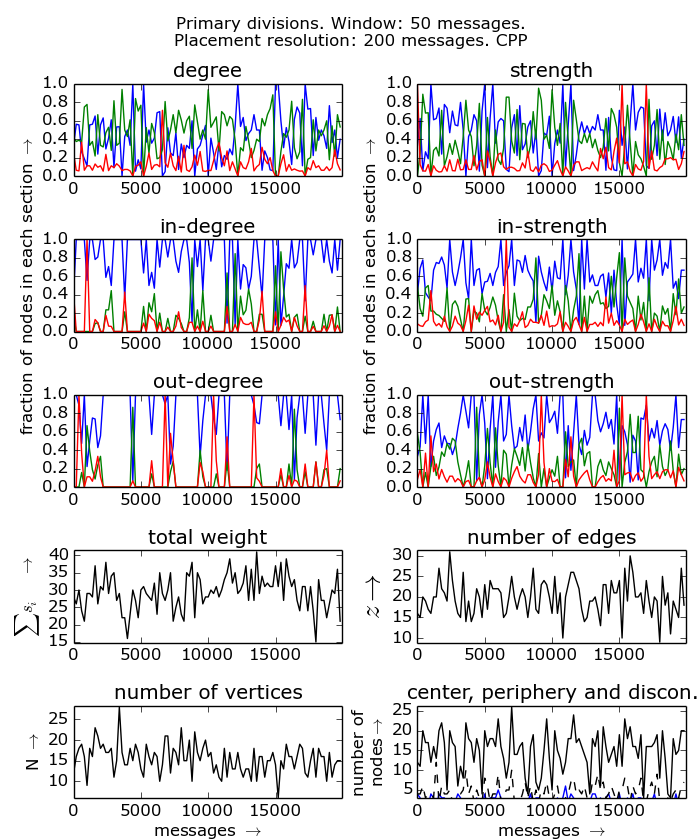
\includegraphics[width=\textwidth]{evoTimelines/evoTimelineCPP-50/CPP-W50-S200}
\end{figure*}
\begin{figure*}
   \centering
        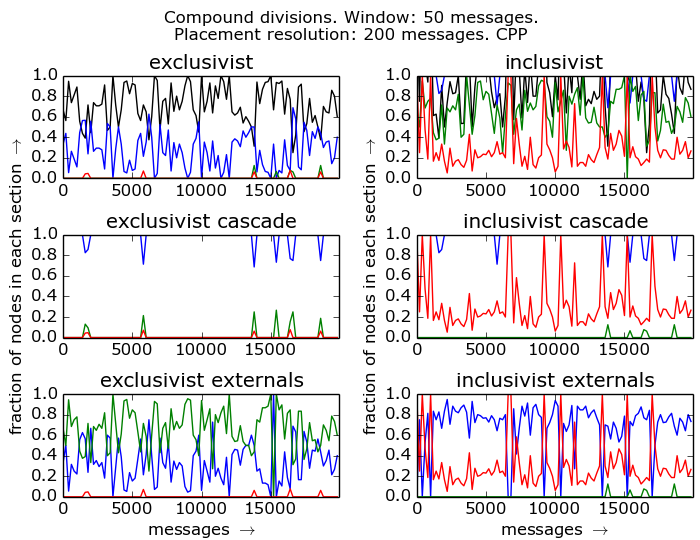
\includegraphics[width=\textwidth]{evoTimelines/evoTimelineCPP-50/CPP-W50-S200_}
\end{figure*}

\begin{figure*}
   \centering
        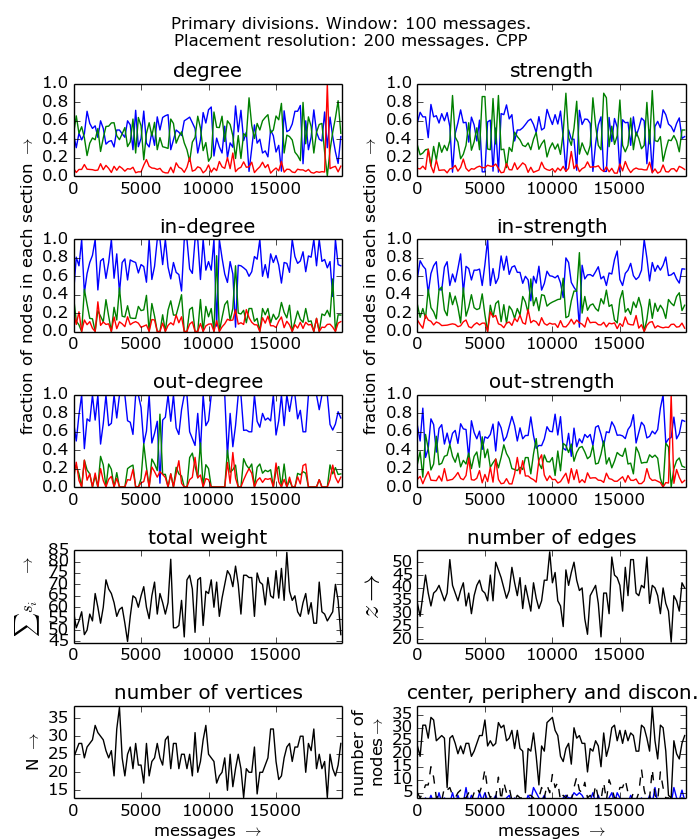
\includegraphics[width=\textwidth]{evoTimelines/evoTimelineCPP-100/CPP-W100-S200}
\end{figure*}
\begin{figure*}
   \centering
        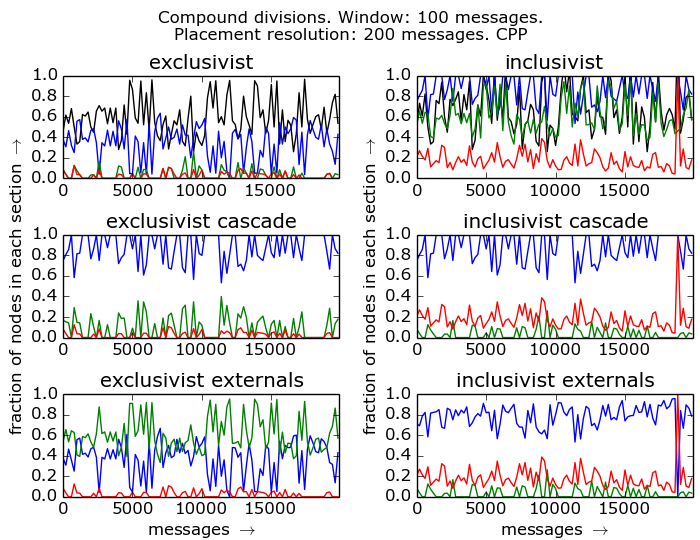
\includegraphics[width=\textwidth]{evoTimelines/evoTimelineCPP-100/CPP-W100-S200_}
\end{figure*}

\begin{figure*}
   \centering
        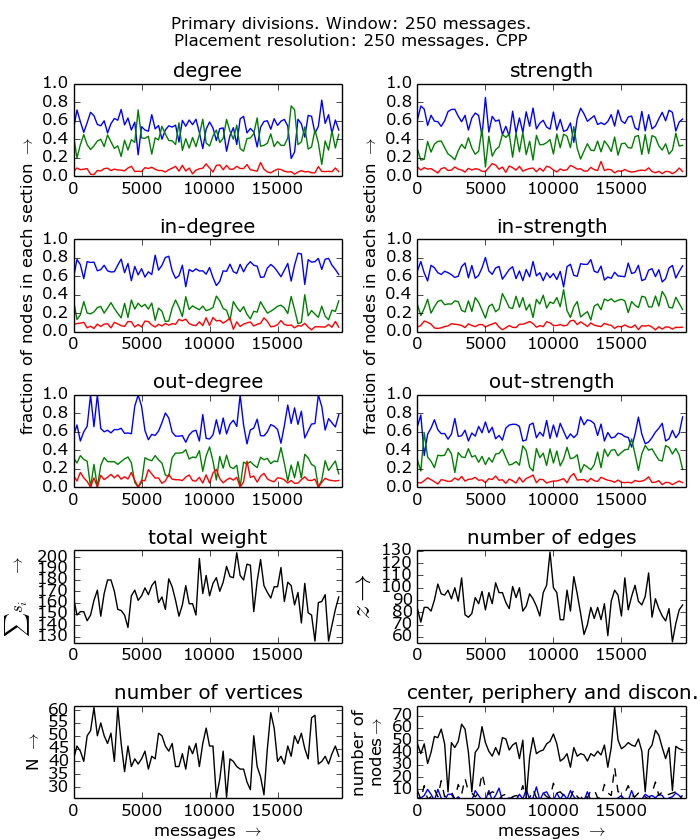
\includegraphics[width=\textwidth]{evoTimelines/evoTimelineCPP-250/CPP-W250-S250}
\end{figure*}
\begin{figure*}
   \centering
        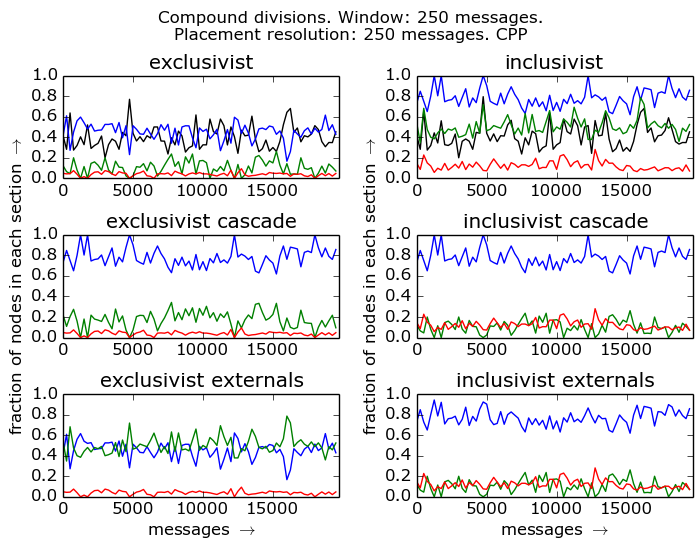
\includegraphics[width=\textwidth]{evoTimelines/evoTimelineCPP-250/CPP-W250-S250_}
\end{figure*}

\begin{figure*}
   \centering
        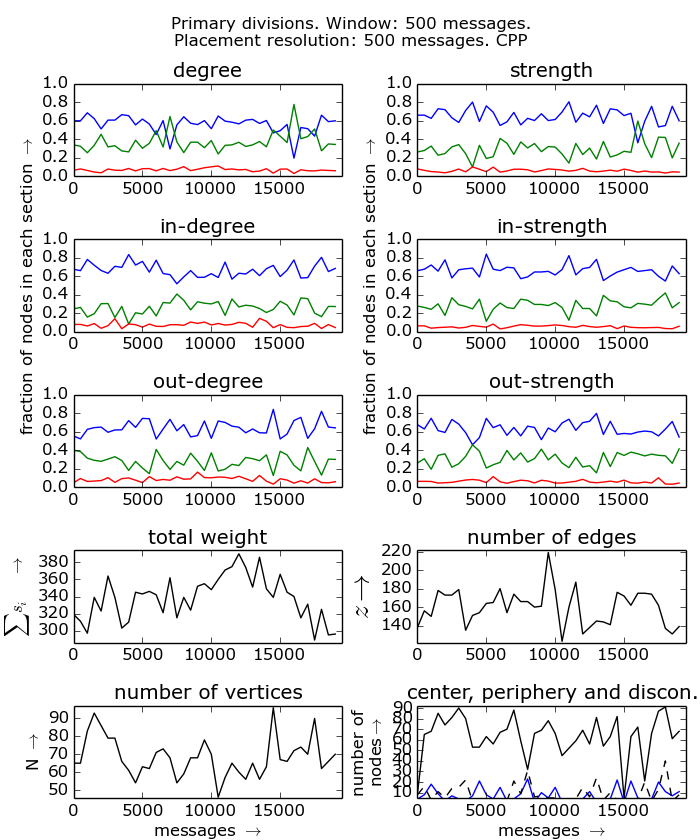
\includegraphics[width=\textwidth]{evoTimelines/evoTimelineCPP-500/CPP-W500-S500}
\end{figure*}
\begin{figure*}
   \centering
        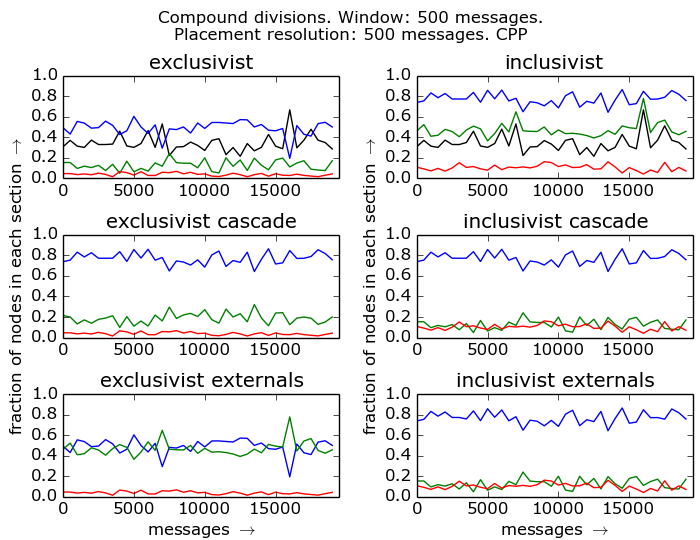
\includegraphics[width=\textwidth]{evoTimelines/evoTimelineCPP-500/CPP-W500-S500_}
\end{figure*}

\begin{figure*}
   \centering
        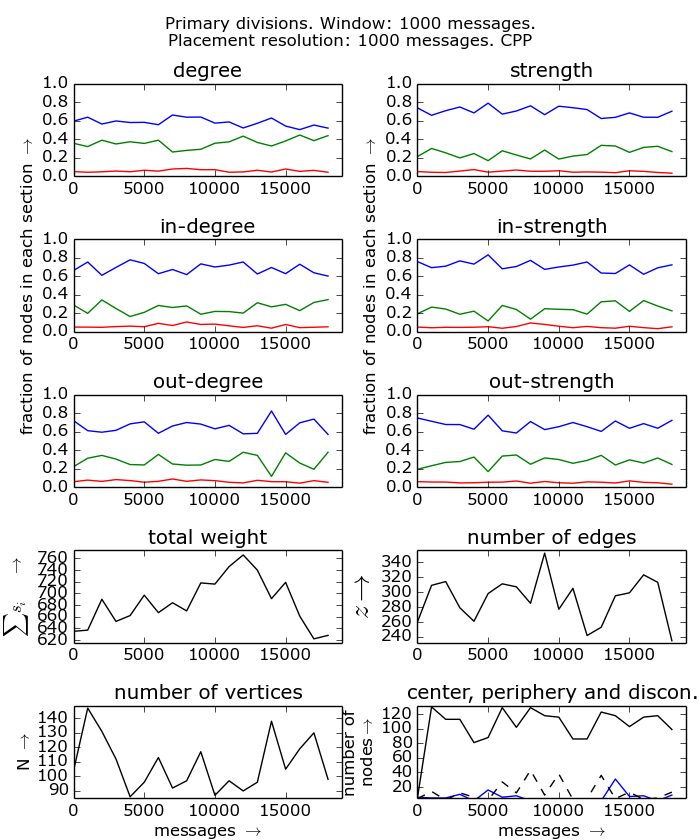
\includegraphics[width=\textwidth]{evoTimelines/evoTimelineCPP-1000/CPP-W1000-S1000}
\end{figure*}
\begin{figure*}
   \centering
        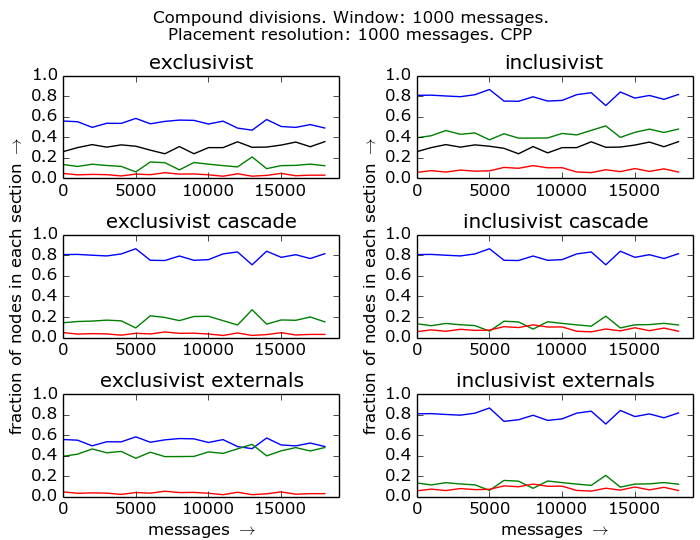
\includegraphics[width=\textwidth]{evoTimelines/evoTimelineCPP-1000/CPP-W1000-S1000_}
\end{figure*}

\begin{figure*}
   \centering
        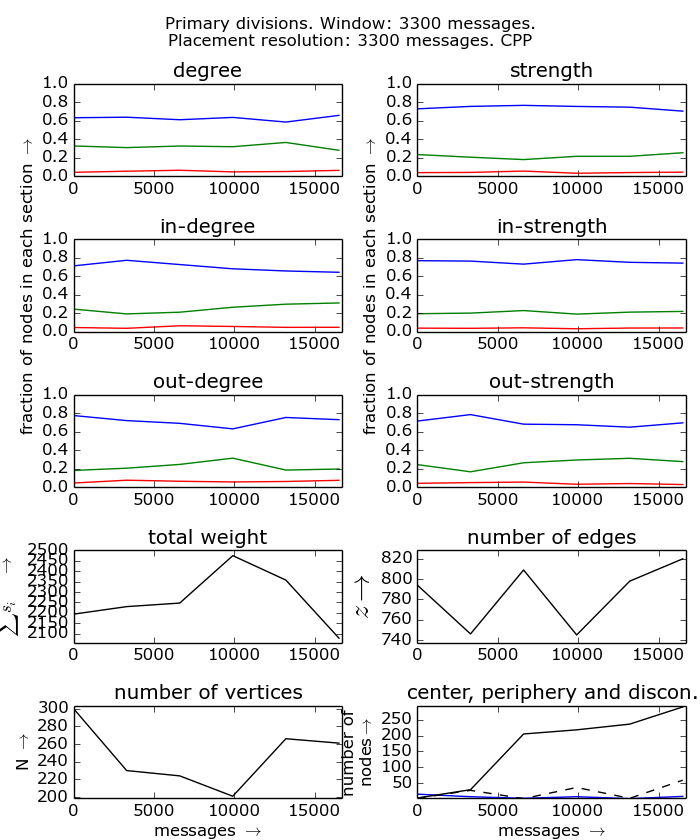
\includegraphics[width=\textwidth]{evoTimelines/evoTimelineCPP-3300/CPP-W3300-S3300}
\end{figure*}
\begin{figure*}
   \centering
   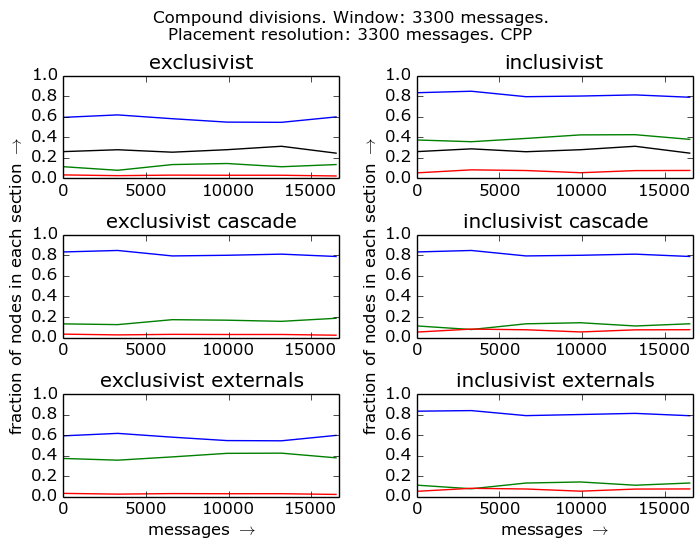
\includegraphics[width=\textwidth]{evoTimelines/evoTimelineCPP-3300/CPP-W3300-S3300_}
\end{figure*}

\begin{figure*}
   \centering
        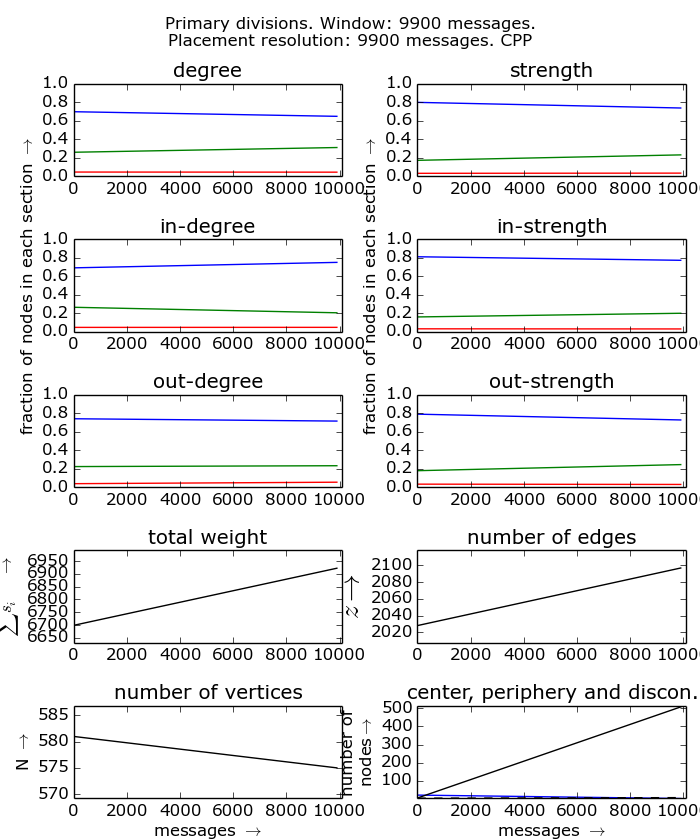
\includegraphics[width=\textwidth]{evoTimelines/evoTimelineCPP-9900/CPP-W9900-S9900}
\end{figure*}
\begin{figure*}
   \centering
   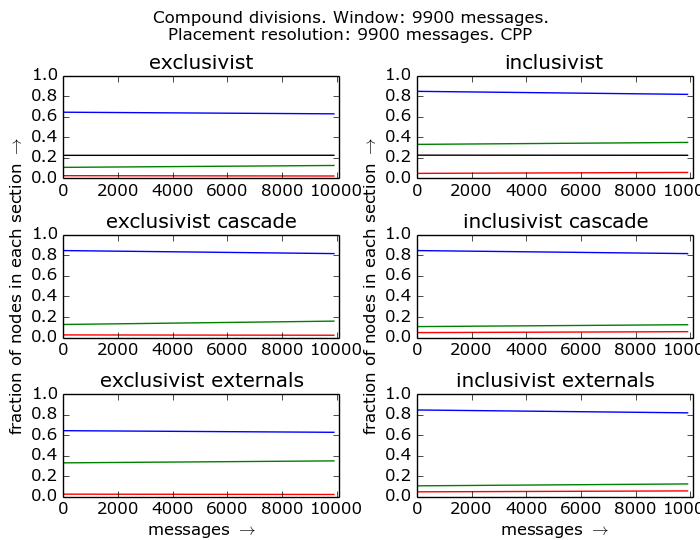
\includegraphics[width=\textwidth]{evoTimelines/evoTimelineCPP-9900/CPP-W9900-S9900_}
\end{figure*}



\FloatBarrier
\subsection{LAD list}

\begin{figure*}
   \centering
        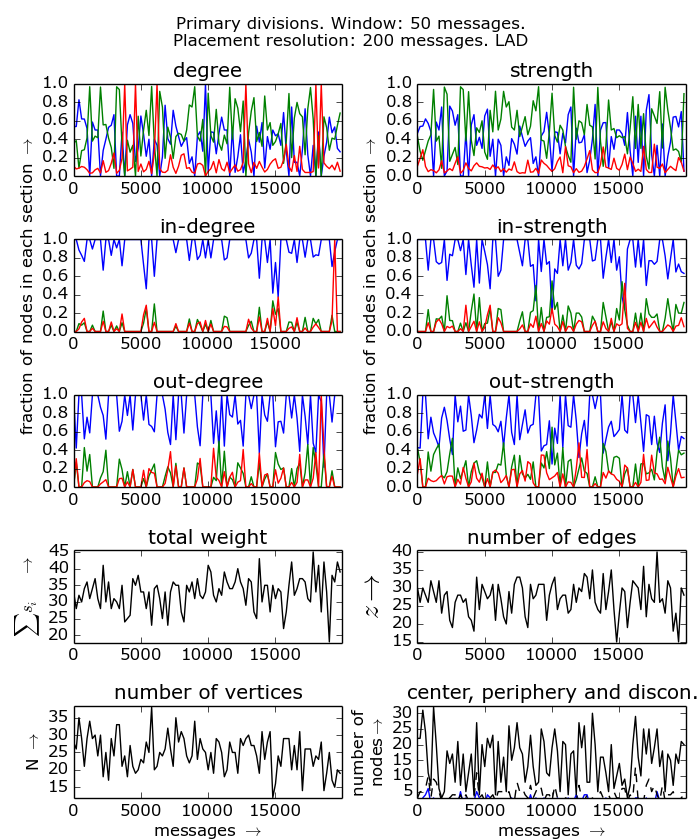
\includegraphics[width=\textwidth]{evoTimelines/evoTimelineLAD-50/LAD-W50-S200}
\end{figure*}
\begin{figure*}
   \centering
        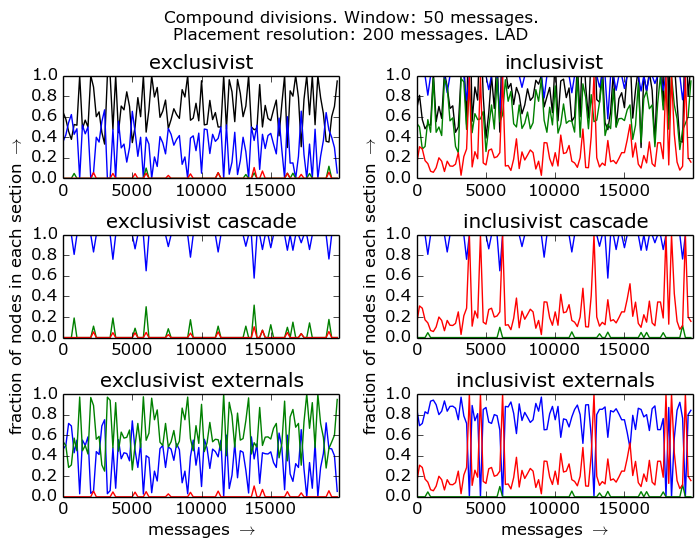
\includegraphics[width=\textwidth]{evoTimelines/evoTimelineLAD-50/LAD-W50-S200_}
\end{figure*}

\begin{figure*}
   \centering
        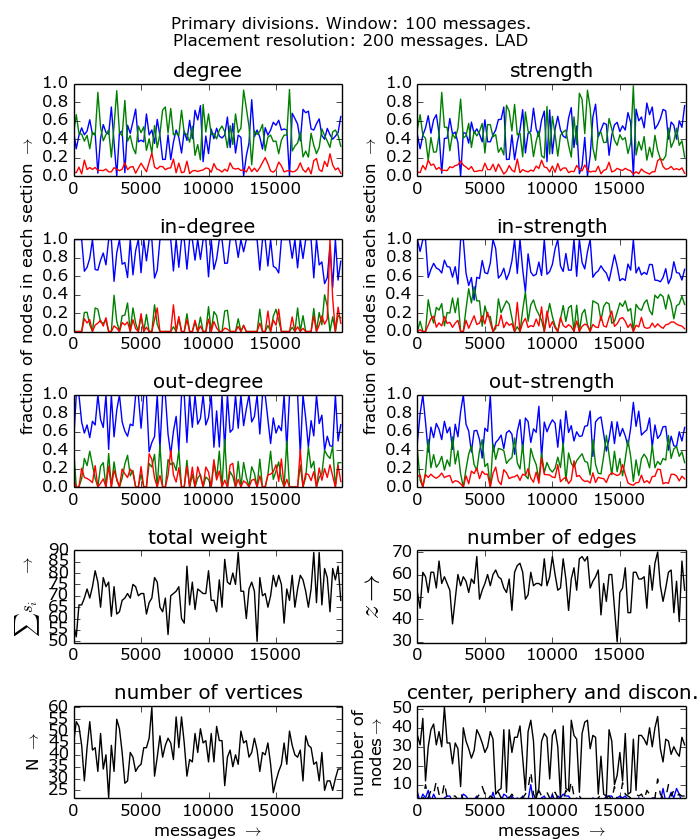
\includegraphics[width=\textwidth]{evoTimelines/evoTimelineLAD-100/LAD-W100-S200}
\end{figure*}
\begin{figure*}
   \centering
        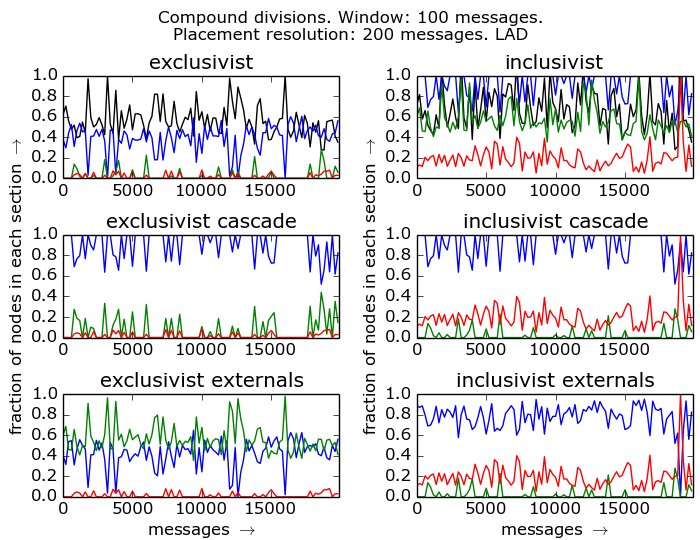
\includegraphics[width=\textwidth]{evoTimelines/evoTimelineLAD-100/LAD-W100-S200_}
\end{figure*}

\begin{figure*}
   \centering
        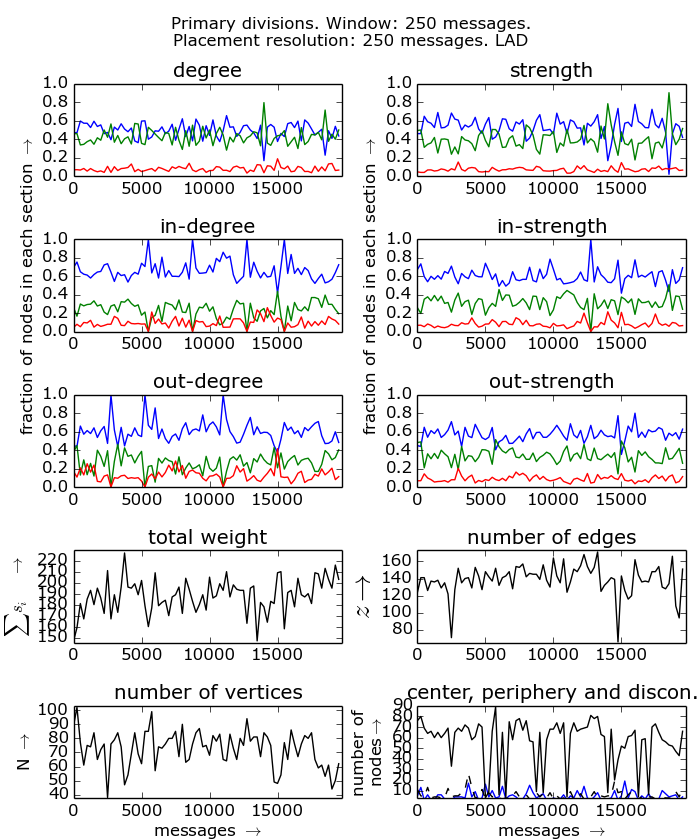
\includegraphics[width=\textwidth]{evoTimelines/evoTimelineLAD-250/LAD-W250-S250}
\end{figure*}
\begin{figure*}
   \centering
        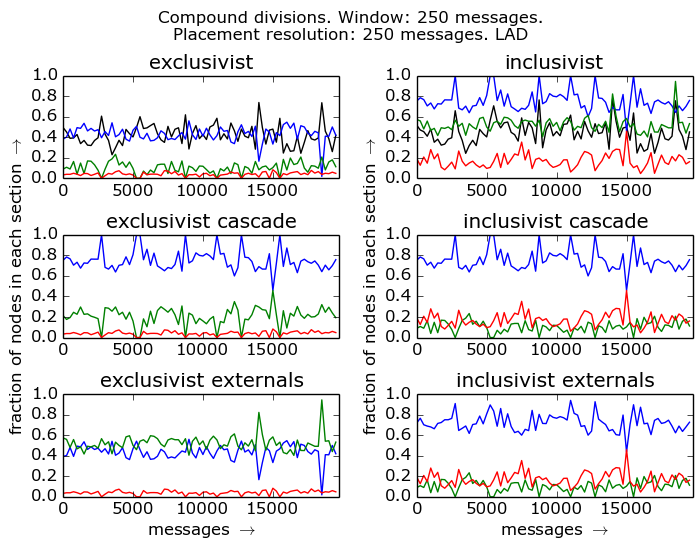
\includegraphics[width=\textwidth]{evoTimelines/evoTimelineLAD-250/LAD-W250-S250_}
\end{figure*}

\begin{figure*}
   \centering
        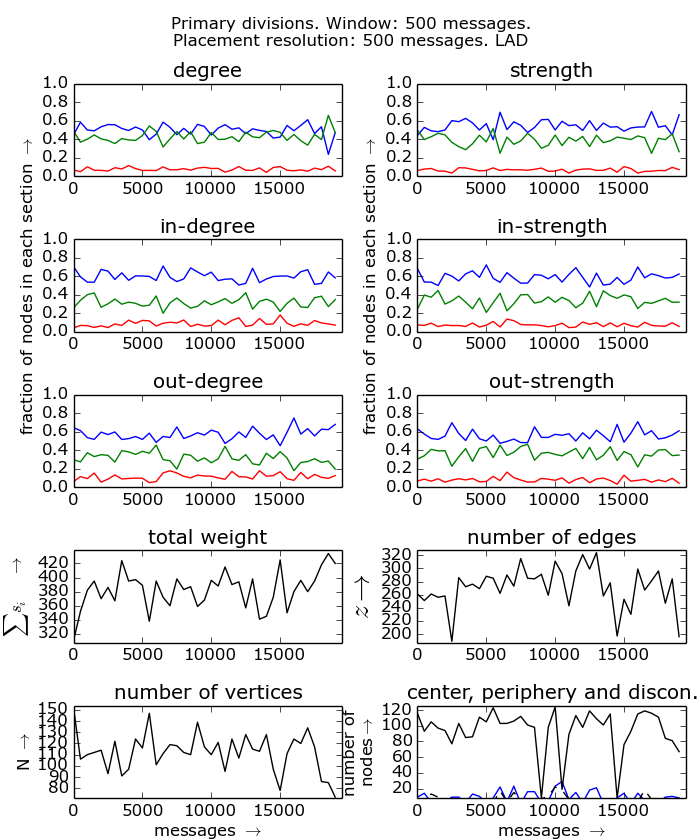
\includegraphics[width=\textwidth]{evoTimelines/evoTimelineLAD-500/LAD-W500-S500}
\end{figure*}
\begin{figure*}
   \centering
        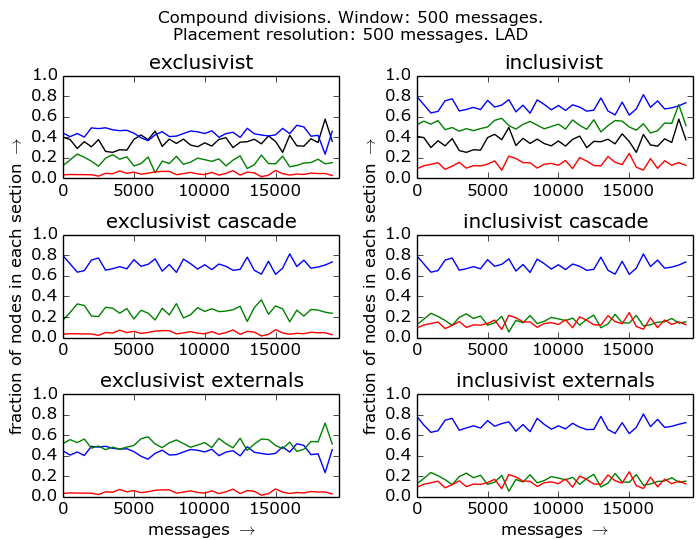
\includegraphics[width=\textwidth]{evoTimelines/evoTimelineLAD-500/LAD-W500-S500_}
\end{figure*}

\begin{figure*}
   \centering
        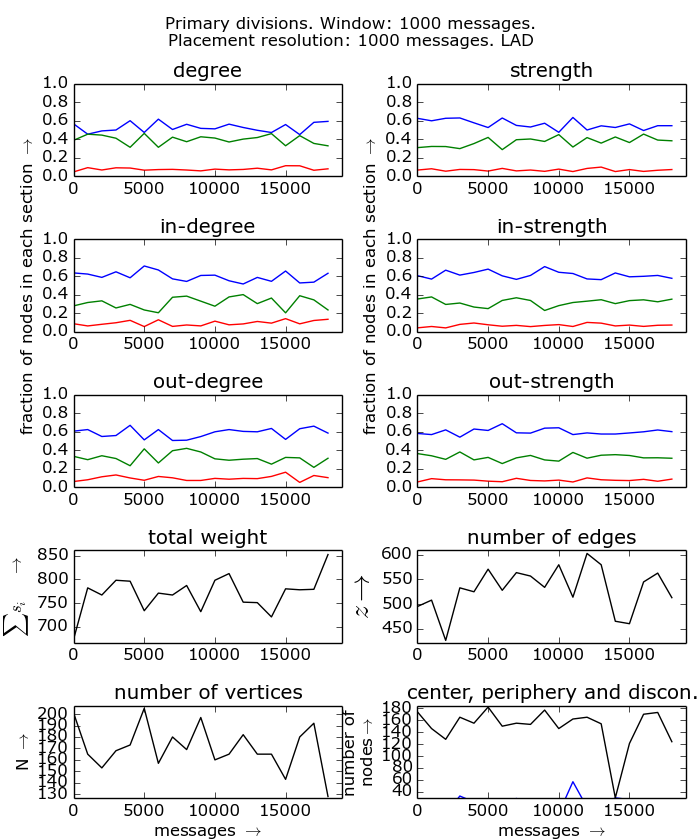
\includegraphics[width=\textwidth]{evoTimelines/evoTimelineLAD-1000/LAD-W1000-S1000}
\end{figure*}
\begin{figure*}
   \centering
        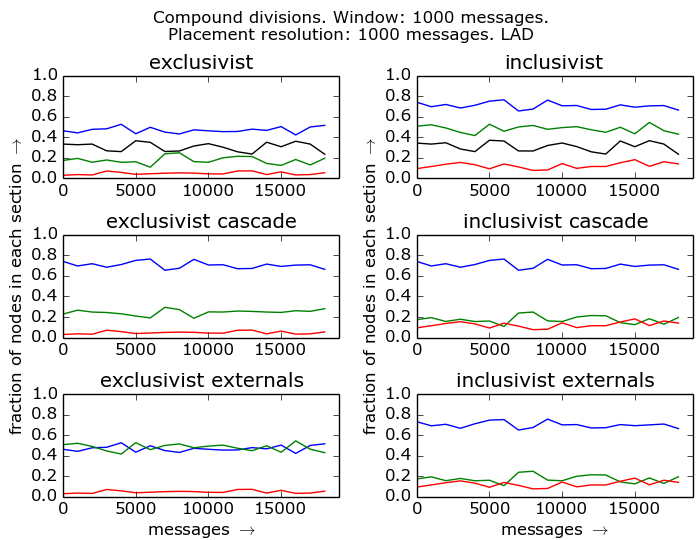
\includegraphics[width=\textwidth]{evoTimelines/evoTimelineLAD-1000/LAD-W1000-S1000_}
\end{figure*}

\begin{figure*}
   \centering
        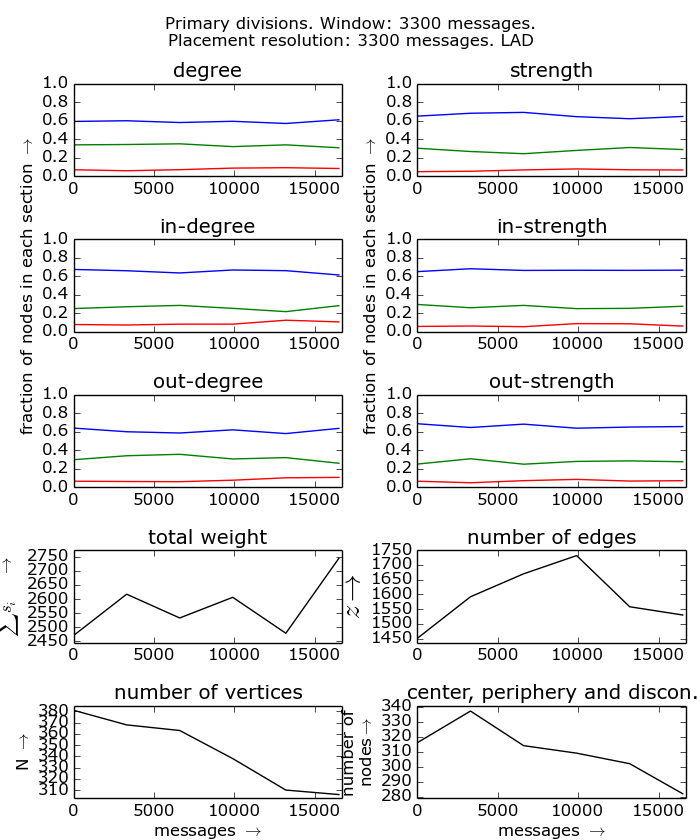
\includegraphics[width=\textwidth]{evoTimelines/evoTimelineLAD-3300/LAD-W3300-S3300}
\end{figure*}
\begin{figure*}
   \centering
        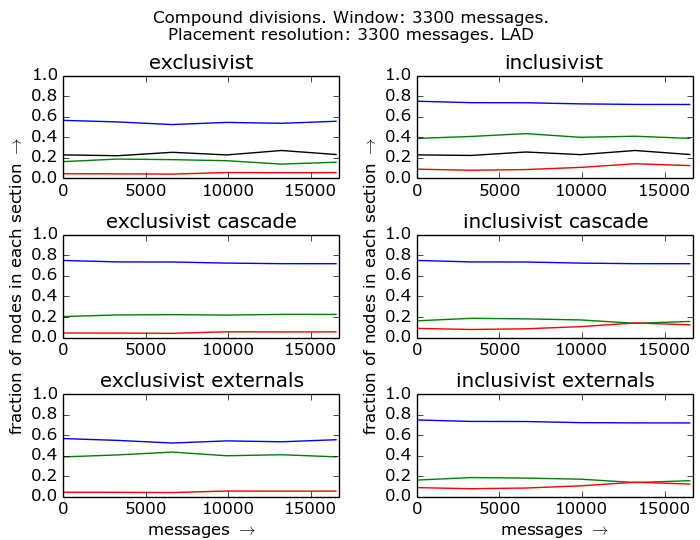
\includegraphics[width=\textwidth]{evoTimelines/evoTimelineLAD-3300/LAD-W3300-S3300_}
\end{figure*}

\begin{figure*}
   \centering
        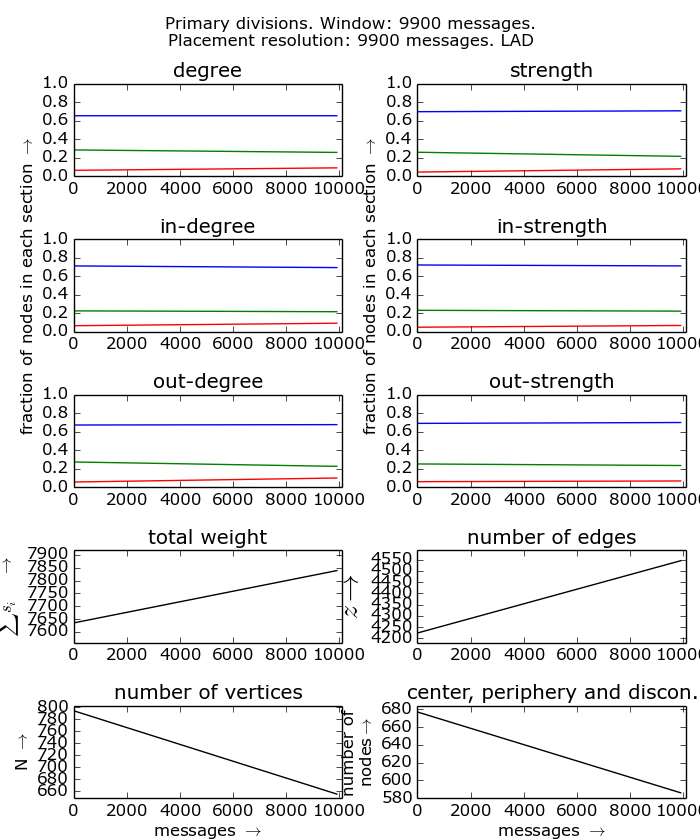
\includegraphics[width=\textwidth]{evoTimelines/evoTimelineLAD-9900/LAD-W9900-S9900}
\end{figure*}
\begin{figure*}
   \centering
        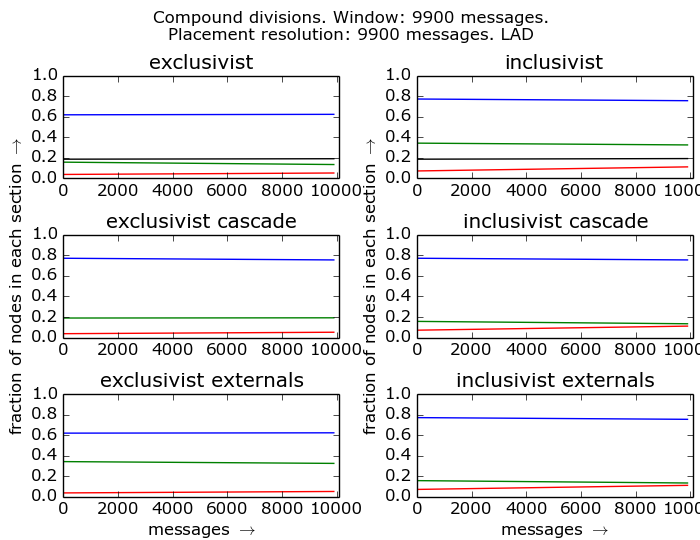
\includegraphics[width=\textwidth]{evoTimelines/evoTimelineLAD-9900/LAD-W9900-S9900_}
\end{figure*}








\FloatBarrier
\section{PCA of measures along the timeline}\label{sec:pcat}
Loadings for the 14 metrics into the principal components for the MET list, $ws=1000$ messages in 20 disjoint positioning. The clustering coefficient (cc) appears as the first metric in the Table, followed by 7 centrality metrics and 6 symmetry-related metrics. Note that the centrality metrics, including degrees, strength and betweenness centrality, are the most important contributors for the first principal component, while the second component is dominated by symmetry metrics. The clustering coefficient is only relevant for the third principal component, coupled with standard deviations of strengths and degrees. The three components have in average 80.36\% of the variance.
\subsection{Betweenness, clustering and degree}

\begin{table}[!h]
	\caption{LAU principal components formation and concentration of dispersion.}
	\footnotesize
	\begin{center}
\begin{tabular}{| l | c | c | c | c | c | c |}\cline{2-7}
\multicolumn{1}{c|}{} & \multicolumn{2}{c|}{PC1}          & \multicolumn{2}{c|}{PC2} & \multicolumn{2}{c|}{PC3}  \\\cline{2-7}\multicolumn{1}{c|}{} & $\mu$            & $\sigma$ & $\mu$         & $\sigma$ & $\mu$ & $\sigma$  \\\hline
$cc$ & 6.03  & 3.73  & 87.60  & 5.25  & 4.52  & 0.93 \\\hline
$k$ & 47.13  & 1.76  & 3.01  & 1.98  & 47.90  & 0.38 \\\hline
$bt$ & 46.84  & 1.97  & 9.39  & 4.31  & 47.58  & 0.57 \\\hline
$\lambda$ & 64.99  & 0.60  & 33.08  & 0.41  & 1.93  & 0.36 \\\hline
\hline\end{tabular}
\end{center}
\label{tab:pcain}
\end{table}

\begin{table}[!h]
	\caption{LAD principal components formation and concentration of dispersion.}
	\footnotesize
	\begin{center}
\begin{tabular}{| l | c | c | c | c | c | c |}\cline{2-7}
\multicolumn{1}{c|}{} & \multicolumn{2}{c|}{PC1}          & \multicolumn{2}{c|}{PC2} & \multicolumn{2}{c|}{PC3}  \\\cline{2-7}\multicolumn{1}{c|}{} & $\mu$            & $\sigma$ & $\mu$         & $\sigma$ & $\mu$ & $\sigma$  \\\hline
$cc$ & 6.42  & 4.05  & 86.60  & 5.50  & 5.19  & 1.45 \\\hline
$k$ & 46.98  & 1.86  & 2.95  & 1.65  & 47.61  & 0.57 \\\hline
$bt$ & 46.59  & 2.18  & 10.45  & 4.72  & 47.20  & 0.90 \\\hline
$\lambda$ & 64.96  & 0.71  & 33.08  & 0.41  & 1.96  & 0.52 \\\hline
\hline\end{tabular}
\end{center}
\label{tab:pcain}
\end{table}

\begin{table}[!h]
	\caption{MET principal components formation and concentration of dispersion.}
	\footnotesize
	\begin{center}
\begin{tabular}{| l || c | c | c | c | c | c |}\cline{2-7}
\multicolumn{1}{c|}{} & \multicolumn{2}{c|}{PC1}          & \multicolumn{2}{c|}{PC2} & \multicolumn{2}{c|}{PC3}  \\\cline{2-7}\multicolumn{1}{c|}{} & $\mu$            & $\sigma$ & $\mu$         & $\sigma$ & $\mu$ & $\sigma$  \\\hline
$cc$ & 5.82  & 3.76  & 87.26  & 5.12  & 4.93  & 1.19 \\
$k$ & 47.18  & 1.82  & 4.35  & 4.01  & 47.63  & 0.57 \\
$bt$ & 47.01  & 1.96  & 8.40  & 4.22  & 47.44  & 0.67 \\\hline\hline
$\lambda$ & 64.94  & 0.76  & 33.13  & 0.45  & 1.93  & 0.62 \\
\hline\end{tabular}
\end{center}

\label{tab:pcain}
\end{table}

\begin{table}[!h]
	\caption{CPP principal components formation and concentration of dispersion.}
	\footnotesize
	\begin{center}
\begin{tabular}{| l | c | c | c | c | c | c |}\cline{2-7}
\multicolumn{1}{c|}{} & \multicolumn{2}{c|}{PC1}          & \multicolumn{2}{c|}{PC2} & \multicolumn{2}{c|}{PC3}  \\\cline{2-7}\multicolumn{1}{c|}{} & $\mu$            & $\sigma$ & $\mu$         & $\sigma$ & $\mu$ & $\sigma$  \\\hline
$cc$ & 3.61  & 2.13  & 91.86  & 3.24  & 3.59  & 0.98 \\\hline
$k$ & 48.24  & 0.99  & 2.96  & 2.25  & 48.25  & 0.43 \\\hline
$bt$ & 48.15  & 1.14  & 5.18  & 3.89  & 48.16  & 0.56 \\\hline
$\lambda$ & 65.24  & 0.51  & 33.30  & 0.17  & 1.46  & 0.49 \\\hline
\hline\end{tabular}
\end{center}
\label{tab:pcain}
\end{table}

\FloatBarrier
\subsection{Betweenness, clustering, degrees and strengths}

\begin{table}[!h]
	\caption{LAU principal components formation and concentration of dispersion.}
	\footnotesize
	\begin{center}
\begin{tabular}{| l || c | c | c | c | c | c |}\cline{2-7}
\multicolumn{1}{c|}{} & \multicolumn{2}{c|}{PC1}          & \multicolumn{2}{c|}{PC2} & \multicolumn{2}{c|}{PC3}  \\\cline{2-7}\multicolumn{1}{c|}{} & $\mu$            & $\sigma$ & $\mu$         & $\sigma$ & $\mu$ & $\sigma$  \\\hline
$cc$ & 1.59  & 0.81  & 80.37  & 5.18  & 3.09  & 1.89 \\\hline
$s$ & 14.40  & 0.15  & 0.81  & 0.68  & 4.75  & 4.43 \\
$s^{in}$ & 14.00  & 0.14  & 2.32  & 1.49  & 18.98  & 4.93 \\
$s^{out}$ & 13.96  & 0.14  & 2.72  & 1.44  & 18.25  & 6.36 \\
$k$ & 14.49  & 0.15  & 0.54  & 0.35  & 1.37  & 0.98 \\
$k^{in}$ & 14.01  & 0.13  & 2.72  & 1.35  & 18.69  & 5.01 \\
$k^{out}$ & 13.85  & 0.13  & 2.37  & 1.73  & 22.63  & 3.79 \\
$bt$ & 13.69  & 0.22  & 8.16  & 1.62  & 12.23  & 8.33 \\\hline\hline
$\lambda$ & 81.87  & 0.88  & 12.48  & 0.15  & 3.33  & 0.70 \\
\hline\end{tabular}
\end{center}

\label{tab:pcain}
\end{table}
\begin{table}[!h]
	\caption{LAD principal components formation and concentration of dispersion.}
	\footnotesize
	\begin{center}
\begin{tabular}{| l | c | c | c | c | c | c |}\cline{2-7}
\multicolumn{1}{c|}{} & \multicolumn{2}{c|}{PC1}          & \multicolumn{2}{c|}{PC2} & \multicolumn{2}{c|}{PC3}  \\\cline{2-7}\multicolumn{1}{c|}{} & $\mu$            & $\sigma$ & $\mu$         & $\sigma$ & $\mu$ & $\sigma$  \\\hline
$cc$ & 1.83  & 1.11  & 80.38  & 11.45  & 3.78  & 4.43 \\\hline
$s$ & 14.25  & 0.17  & 1.34  & 1.81  & 9.88  & 5.76 \\
$s^{in}$ & 13.99  & 0.19  & 2.06  & 1.70  & 17.62  & 6.15 \\
$s^{out}$ & 14.03  & 0.22  & 1.81  & 1.98  & 15.44  & 6.68 \\
$k$ & 14.38  & 0.13  & 0.95  & 1.64  & 3.45  & 3.15 \\
$k^{in}$ & 14.05  & 0.14  & 2.26  & 1.66  & 13.44  & 7.26 \\
$k^{out}$ & 13.96  & 0.15  & 1.72  & 1.53  & 16.14  & 6.37 \\
$bt$ & 13.51  & 0.35  & 9.48  & 2.86  & 20.26  & 9.87 \\\hline\hline
$\lambda$ & 82.32  & 1.61  & 12.52  & 0.26  & 2.97  & 1.21 \\
\hline\end{tabular}
\end{center}
\label{tab:pcain}
\end{table}
\begin{table}[!h]
	\caption{MET principal components formation and concentration of dispersion.}
	\footnotesize
	\begin{center}
\begin{tabular}{| l | c | c | c | c | c | c |}\cline{2-7}
\multicolumn{1}{c|}{} & \multicolumn{2}{c|}{PC1}          & \multicolumn{2}{c|}{PC2} & \multicolumn{2}{c|}{PC3}  \\\cline{2-7}\multicolumn{1}{c|}{} & $\mu$            & $\sigma$ & $\mu$         & $\sigma$ & $\mu$ & $\sigma$  \\\hline
$cc$ & 1.16  & 0.76  & 81.72  & 3.00  & 1.61  & 1.78 \\\hline
$s$ & 14.32  & 0.16  & 1.76  & 1.12  & 11.39  & 5.50 \\
$s^{in}$ & 14.17  & 0.11  & 2.29  & 1.29  & 14.46  & 3.72 \\
$s^{out}$ & 14.09  & 0.17  & 1.72  & 1.18  & 17.54  & 5.37 \\
$k$ & 14.39  & 0.16  & 1.73  & 0.63  & 4.76  & 2.82 \\
$k^{in}$ & 14.12  & 0.13  & 1.02  & 0.71  & 11.69  & 6.93 \\
$k^{out}$ & 14.06  & 0.13  & 3.11  & 1.58  & 12.18  & 9.24 \\
$bt$ & 13.69  & 0.26  & 6.64  & 2.01  & 26.37  & 12.37 \\\hline\hline
$\lambda$ & 83.41  & 1.53  & 12.53  & 0.11  & 2.34  & 1.16 \\
\hline\end{tabular}
\end{center}
\label{tab:pcain}
\end{table}
\begin{table}[!h]
	\caption{CPP principal components formation and concentration of dispersion.}
	\footnotesize
	\begin{center}
\begin{tabular}{| l | c | c | c | c | c | c |}\cline{2-7}
\multicolumn{1}{c|}{} & \multicolumn{2}{c|}{PC1}          & \multicolumn{2}{c|}{PC2} & \multicolumn{2}{c|}{PC3}  \\\cline{2-7}\multicolumn{1}{c|}{} & $\mu$            & $\sigma$ & $\mu$         & $\sigma$ & $\mu$ & $\sigma$  \\\hline
$cc$ & 0.84  & 0.61  & 80.59  & 6.89  & 2.30  & 2.19 \\\hline
$s$ & 14.28  & 0.07  & 0.97  & 1.03  & 15.89  & 1.15 \\
$s^{in}$ & 14.18  & 0.12  & 2.89  & 1.71  & 13.50  & 5.19 \\
$s^{out}$ & 14.07  & 0.23  & 2.83  & 1.63  & 18.80  & 4.94 \\
$k$ & 14.42  & 0.08  & 0.78  & 0.67  & 7.48  & 2.71 \\
$k^{in}$ & 14.29  & 0.10  & 2.36  & 1.41  & 7.21  & 4.49 \\
$k^{out}$ & 14.16  & 0.12  & 3.62  & 1.83  & 8.79  & 4.58 \\
$bt$ & 13.76  & 0.22  & 5.96  & 1.88  & 26.03  & 7.94 \\\hline\hline
$\lambda$ & 83.32  & 1.42  & 12.60  & 0.08  & 2.61  & 1.15 \\
\hline\end{tabular}
\end{center}
\label{tab:pcain}
\end{table}


\FloatBarrier
\subsection{Betweenness, clustering, degrees, strengths and symmetry measures}

\begin{table}[!h]
	\caption{LAU principal components formation and concentration of dispersion.}
	\footnotesize
	\begin{center}
\begin{tabular}{| l | c | c | c | c | c | c |}\cline{2-7}
\multicolumn{1}{c|}{} & \multicolumn{2}{c|}{PC1}          & \multicolumn{2}{c|}{PC2} & \multicolumn{2}{c|}{PC3}  \\\cline{2-7}\multicolumn{1}{c|}{} & $\mu$            & $\sigma$ & $\mu$         & $\sigma$ & $\mu$ & $\sigma$  \\\hline
$cc$ & 1.64  & 0.77  & 2.42  & 1.71  & 19.20  & 3.96 \\\hline
$s$ & 12.80  & 0.46  & 0.89  & 0.82  & 2.53  & 0.63 \\
$s^{in}$ & 12.47  & 0.42  & 2.30  & 0.97  & 2.29  & 0.81 \\
$s^{out}$ & 12.37  & 0.46  & 2.89  & 1.24  & 2.64  & 0.58 \\
$k$ & 12.93  & 0.44  & 0.82  & 0.73  & 1.32  & 0.45 \\
$k^{in}$ & 12.54  & 0.37  & 2.88  & 1.13  & 1.02  & 0.56 \\
$k^{out}$ & 12.32  & 0.46  & 3.82  & 1.14  & 1.57  & 0.68 \\
$bt$ & 12.19  & 0.46  & 1.06  & 0.62  & 2.64  & 0.89 \\\hline
$asy$ & 0.93  & 0.81  & 20.38  & 0.82  & 1.66  & 1.09 \\
$\mu^{asy}$ & 0.96  & 0.83  & 20.26  & 0.82  & 1.66  & 1.04 \\
$\sigma^{asy}$ & 6.18  & 0.71  & 1.24  & 0.92  & 27.98  & 1.74 \\
$dis$ & 0.90  & 0.79  & 20.36  & 0.82  & 1.54  & 1.07 \\
$\mu^{dis}$ & 0.92  & 0.61  & 19.02  & 0.84  & 1.45  & 1.12 \\
$\sigma^{dis}$ & 0.86  & 0.51  & 1.64  & 1.10  & 32.51  & 1.90 \\
$\lambda$ & 48.41  & 0.52  & 27.95  & 0.36  & 12.81  & 0.79 \\
\hline\end{tabular}
\end{center}
\label{tab:pcain}
\end{table}
\begin{table}[!h]
	\caption{LAD principal components formation and concentration of dispersion.}
	\footnotesize
	\begin{center}
\begin{tabular}{| l | c | c | c | c | c | c |}\cline{2-7}
\multicolumn{1}{c|}{} & \multicolumn{2}{c|}{PC1}          & \multicolumn{2}{c|}{PC2} & \multicolumn{2}{c|}{PC3}  \\\cline{2-7}\multicolumn{1}{c|}{} & $\mu$            & $\sigma$ & $\mu$         & $\sigma$ & $\mu$ & $\sigma$  \\\hline
$cc$ & 1.96  & 0.95  & 3.07  & 1.46  & 17.94  & 5.38 \\\hline
$s$ & 12.34  & 0.57  & 1.72  & 0.99  & 2.43  & 0.93 \\
$s^{in}$ & 12.06  & 0.64  & 3.18  & 0.98  & 1.98  & 1.09 \\
$s^{out}$ & 12.22  & 0.48  & 1.14  & 0.78  & 2.83  & 0.79 \\
$k$ & 12.54  & 0.56  & 1.43  & 0.87  & 0.92  & 0.44 \\
$k^{in}$ & 12.15  & 0.61  & 3.81  & 0.79  & 0.61  & 0.42 \\
$k^{out}$ & 12.27  & 0.45  & 1.51  & 1.08  & 1.56  & 0.39 \\
$bt$ & 11.73  & 0.64  & 1.80  & 0.88  & 2.28  & 1.00 \\\hline
$asy$ & 1.51  & 0.97  & 19.66  & 1.63  & 3.02  & 1.66 \\
$\mu_{asy}$ & 1.41  & 0.99  & 19.53  & 1.62  & 3.00  & 1.69 \\
$\sigma_{asy}$ & 5.62  & 0.68  & 2.01  & 1.23  & 27.46  & 3.31 \\
$dis$ & 1.58  & 0.98  & 19.57  & 1.65  & 3.21  & 1.71 \\
$\mu_{dis}$ & 1.84  & 1.00  & 18.62  & 1.52  & 2.08  & 1.13 \\
$\sigma_{dis}$ & 0.77  & 0.59  & 2.94  & 1.60  & 30.68  & 3.34 \\\hline\hline
$\lambda$ & 48.65  & 1.03  & 27.84  & 0.31  & 13.00  & 0.77 \\
\hline\end{tabular}
\end{center}
\label{tab:pcain}
\end{table}
\begin{table}[!h]
	\caption{MET principal components formation and concentration of dispersion.}
	\footnotesize
	\begin{center}
\begin{tabular}{| l || c | c | c | c | c | c |}\cline{2-7}
\multicolumn{1}{c|}{} & \multicolumn{2}{c|}{PC1}          & \multicolumn{2}{c|}{PC2} & \multicolumn{2}{c|}{PC3}  \\\cline{2-7}\multicolumn{1}{c|}{} & $\mu$            & $\sigma$ & $\mu$         & $\sigma$ & $\mu$ & $\sigma$  \\\hline
$cc$ & 1.18  & 0.71  & 3.00  & 2.35  & 22.39  & 2.71 \\\hline
$s$ & 12.34  & 0.66  & 1.74  & 1.17  & 1.55  & 0.75 \\
$s^{in}$ & 12.25  & 0.62  & 1.74  & 0.96  & 1.45  & 0.77 \\
$s^{out}$ & 12.11  & 0.72  & 2.42  & 1.35  & 1.78  & 0.78 \\
$k$ & 12.48  & 0.63  & 1.46  & 0.91  & 0.54  & 0.48 \\
$k^{in}$ & 12.32  & 0.56  & 1.54  & 1.22  & 0.65  & 0.62 \\
$k^{out}$ & 12.12  & 0.67  & 3.10  & 1.15  & 0.87  & 0.74 \\
$bt$ & 11.85  & 0.62  & 1.46  & 0.87  & 1.16  & 0.70 \\\hline
$asy$ & 1.79  & 1.22  & 19.35  & 2.15  & 3.29  & 2.15 \\
$\mu^{asy}$ & 1.84  & 1.22  & 19.17  & 2.16  & 3.31  & 2.23 \\
$\sigma^{asy}$ & 4.17  & 0.79  & 3.91  & 2.35  & 27.79  & 3.96 \\
$dis$ & 1.78  & 1.18  & 19.26  & 2.15  & 3.38  & 2.29 \\
$\mu^{dis}$ & 1.53  & 1.10  & 18.23  & 2.12  & 3.32  & 1.71 \\
$\sigma^{dis}$ & 2.23  & 0.93  & 3.61  & 2.38  & 28.54  & 3.23 \\\hline\hline
$\lambda$ & 49.05  & 1.01  & 27.79  & 0.30  & 13.30  & 1.35 \\
\hline\end{tabular}
\end{center}

\label{tab:pcain}
\end{table}
\begin{table}[!h]
	\caption{CPP principal components formation and concentration of dispersion.}
	\footnotesize
	\begin{center}
\begin{tabular}{| l | c | c | c | c | c | c |}\cline{2-7}
\multicolumn{1}{c|}{} & \multicolumn{2}{c|}{PC1}          & \multicolumn{2}{c|}{PC2} & \multicolumn{2}{c|}{PC3}  \\\cline{2-7}\multicolumn{1}{c|}{} & $\mu$            & $\sigma$ & $\mu$         & $\sigma$ & $\mu$ & $\sigma$  \\\hline
$cc$ & 0.89  & 0.59  & 1.93  & 1.33  & 21.22  & 2.97 \\\hline
$s$ & 11.71  & 0.57  & 2.97  & 0.82  & 2.45  & 0.72 \\
$s^{in}$ & 11.68  & 0.58  & 2.37  & 0.91  & 3.08  & 0.78 \\
$s^{out}$ & 11.49  & 0.61  & 3.63  & 0.79  & 1.61  & 0.88 \\
$k$ & 11.93  & 0.54  & 2.58  & 0.70  & 0.52  & 0.44 \\
$k^{in}$ & 11.93  & 0.52  & 1.19  & 0.88  & 1.41  & 0.71 \\
$k^{out}$ & 11.57  & 0.61  & 4.34  & 0.70  & 0.98  & 0.66 \\
$bt$ & 11.37  & 0.55  & 2.44  & 0.84  & 1.37  & 0.77 \\\hline
$asy$ & 3.14  & 0.98  & 18.52  & 1.97  & 2.46  & 1.69 \\
$\mu^{asy}$ & 3.32  & 0.99  & 18.23  & 2.01  & 2.80  & 1.82 \\
$\sigma^{asy}$ & 4.91  & 0.59  & 2.44  & 1.47  & 26.84  & 3.06 \\
$dis$ & 2.94  & 0.88  & 18.50  & 1.92  & 3.06  & 1.98 \\
$\mu^{dis}$ & 2.55  & 0.89  & 18.12  & 1.85  & 1.57  & 1.32 \\
$\sigma^{dis}$ & 0.57  & 0.33  & 2.74  & 1.63  & 30.61  & 2.66 \\\hline\hline
$\lambda$ & 49.56  & 1.16  & 27.14  & 0.54  & 13.25  & 0.95 \\
\hline\end{tabular}
\end{center}

\label{tab:pcain}
\end{table}


\section{Stability in other networks: Twitter, Facebook, Participa.br}\label{sec:pcat}
To further verify the hypothesis that such stability is a general property of human social networks,
we analyzed networks driven from Twitter, Facebook and Participa.br. Selected networks are summarized in
Table~\ref{tab:E}. Their Erd\"os sector relative sizes are given in Table~\ref{tab:secE}. PCA formations are given in
Tables~\ref{tab:pcaE1I},~\ref{tab:pcaE1F},~\ref{tab:pcaE2} and~\ref{tab:pcaE3}. Friendship networks considered are undirected and unweighted,
therefore all measures of strength, in- and out- centralities, asymmetry and disequilibrium have little or no meaning, which is why F1, F2, F3, F4 and F5 are only present in Table~\ref{tab:pcaE1F}.

\begin{table*}[!h]
	\caption{Overview of selected networks analyzed in addition to email interaction networks. Three social platforms were the sources of network structures: Facebook, Twitter and Participa.br. Both friendship and interaction networks were observed, yielding undirected and directed networks, respectively. The number of agents $N$ and the number of edges $z$ are given on the last columns. The acronyms are used throughout Tables~\ref{tab:secE},~\ref{tab:pcaE1I},~\ref{tab:pcaE1F},~\ref{tab:pcaE2} and~\ref{tab:pcaE3}. All these network data were collected in 2013 and 2014.}
\begin{center}
\begin{tabular}{| l | c | c | c | c | c | c | }\hline
	acronym & provenance & edge & directed & description & $N$ & $z$ \\ \hline\hline
	F1 & Facebook  & friendship  & no  & the friendship network of Renato Fabbri (author)  & 1367  & 28606 \\\hline
F2 & Facebook  & friendship  & no  & the friendship network of Massimo Canevacci (senior anthropologist)  & 4764  & 59995 \\\hline
F3 & Facebook  & friendship  & no  & the friendship network of a brazilian direct democracy group  & 3599  & 59471 \\\hline
F4 & Facebook  & friendship  & no  & the friendship network of the Silicon Valley Global Network group  & 2026  & 15586 \\\hline
F5 & Participa.br  & friendship  & no  & the friendship network of a brazilian federal social participation portal  & 443  & 910 \\\hline
I1 & Facebook  & interaction  & yes  & the interaction network of the Silicon Valley Global Network group  & 104  & 154 \\\hline
I2 & Facebook  & interaction  & yes  & the interaction network of a Solidarity Economy group  & 64  & 120 \\\hline
I3 & Facebook  & interaction  & yes  & the interaction network of a brazilian direct democracy group  & 214  & 310 \\\hline
I4 & Facebook  & interaction  & yes  & the interaction network of the 'Cience with Frontiers' group  & 530  & 1658 \\\hline
I5 & Participa.br  & interaction  & yes  & the interaction network of a brazilian federal social participation portal  & 222  & 300 \\\hline
TT1 & Twitter  & retweet  & yes  & the retweet network of $\approx 22k$ tweets with the hashtag \#arenaNETmundial  & 2772  & 7222 \\\hline
TT2 & Twitter  & retweet  & yes  & same as TT1, but disconnected agents are not discarded  & 2975  & 7222 \\\hline

\hline
\end{tabular}
\end{center}
\label{tab:E}
\end{table*}


\begin{table*}[!h]
	\caption{Percentage of agents in each Erd\"os sector in the friendship and interaction human networks of Table~\ref{tab:E}. The ratios found in email networks are preserved. Most notable exceptions are I1 and I4, which might be understood as outliers, A possible explanation for them is that they might be a system better characterized as a superposition of networks, rather than one coherent network.}
\begin{center}
\begin{tabular}{| l | c | c | c |}\hline
	 & periphery & intermediary & hubs \\ \hline\hline
	F1 & 53.11  & 43.31  & 3.58 \\\hline
F2 & 58.98  & 39.29  & 1.72 \\\hline
F3 & 65.41  & 31.87  & 2.72 \\\hline
F4 & 66.49  & 32.03  & 1.48 \\\hline
F5 & 62.98  & 36.12  & 0.90 \\\hline
I1 & 4.81  & 94.23  & 0.96 \\\hline
I2 & 53.12  & 45.31  & 1.56 \\\hline
I3 & 58.41  & 40.19  & 1.40 \\\hline
I4 & 39.06  & 59.43  & 1.51 \\\hline
I5 & 54.95  & 43.69  & 1.35 \\\hline
TT1 & 74.86  & 24.49  & 0.65 \\\hline
TT2 & 76.57  & 22.86  & 0.57 \\\hline

\hline
\end{tabular}
\end{center}
\label{tab:secE}
\end{table*}


\begin{table*}[!h]
	\caption{First three principal components formation and variance concentration for each of the five friendship networks of Table~\ref{tab:E} in the simplest case: dimensions correspond to degree, clustering coefficient and betweenness centrality. Participa.br yields the networks that most resembles email networks. Overall, the general characteristic is preserved: first component is an average of degree and betweenness, while clustering is the most relevant for second component. The friendship of Renato Fabbri (F1) is the only whose first component has more than 20\% of custering coefficient and second component has more than 40\% of degree centrality.}
	\footnotesize
\begin{center}
%\begin{tabular}{| l | c |c |c |c |c |c |c |c |c |c |c |c |c |c |c |c |c |c |c |c |c |c |c |c |c |c |c |c |c |c |c |c |c | c | c | c |}\hline
\begin{tabular}{| l ||  c |c |c |c |c || c | c | c | c | c || c |c |c |c |c |	}\cline{2-16}
%	 & p. & i. & h. \\ \hline\hline
\multicolumn{1}{c|}{} & \multicolumn{5}{c||}{PC1}          & \multicolumn{5}{c||}{PC2} & \multicolumn{5}{c|}{PC3}  \\\cline{2-16}
	\multicolumn{1}{c|}{} & 
	F1 & F2 & F3 & F4 & F5 &	
	F1 & F2 & F3 & F4 & F5 &	
	F1 & F2 & F3 & F4 & F5 	\\\hline
	$cc$ & 25.80  & 12.22  & 11.54  & 5.04  & 0.94  & 58.87  & 78.22  & 68.86  & 90.39  & 88.86  & 6.95  & 1.13  & 18.20  & 3.02  & 5.90 \\
$k$ & 36.43  & 43.96  & 45.61  & 47.40  & 49.50  & 25.66  & 9.98  & 6.10  & 7.63  & 6.42  & 44.94  & 49.52  & 42.00  & 48.41  & 47.02 \\
$bt$ & 37.77  & 43.82  & 42.85  & 47.56  & 49.56  & 15.46  & 11.80  & 25.04  & 1.98  & 4.72  & 48.11  & 49.35  & 39.80  & 48.57  & 47.08 \\\hline\hline
$\lambda$ & 53.15  & 53.06  & 46.26  & 55.36  & 63.80  & 28.69  & 32.57  & 34.27  & 33.25  & 33.57  & 18.16  & 14.37  & 19.47  & 11.38  & 2.63 \\

\hline
\end{tabular}
\end{center}
\label{tab:pcaE1F}
\end{table*}


\begin{table*}[!h]
	\caption{First three principal components formation and variance concentration for each of the seven interaction networks of Table~\ref{tab:E} in the simplest case: dimensions correspond to degree, clustering coefficient and betweenness centrality. Twitter yields the networks that most resembles email networks. Overall, the general characteristic is preserved: first component is an average of degree and betweenness, while clustering is the most relevant for second component.}
	\footnotesize
\begin{center}
%\begin{tabular}{| l | c |c |c |c |c |c |c |c |c |c |c |c |c |c |c |c |c |c |c |c |c |c |c |c |c |c |c |c |c |c |c |c |c | c | c | c |}\hline
\begin{tabular}{| l ||  c |c |c |c |c | c | c || c | c | c | c | c | c | c || c |c |c |c |c | c | c |	}\cline{2-22}
%	 & p. & i. & h. \\ \hline\hline
\multicolumn{1}{c|}{} & \multicolumn{7}{c||}{PC1}          & \multicolumn{7}{c||}{PC2} & \multicolumn{7}{c|}{PC3}  \\\cline{2-22}
	\multicolumn{1}{c|}{} & 
	I1 & I2 & I3 & I4 & I5 & TT1 & TT2 &
	I1 & I2 & I3 & I4 & I5 & TT1 & TT2 &
	I1 & I2 & I3 & I4 & I5 & TT1 & TT2 \\\hline
	$cc$ & 14.43  & 17.12  & 11.54  & 0.69  & 13.26  & 2.17  & 2.72  & 74.78  & 70.72  & 79.30  & 96.63  & 76.59  & 95.75  & 94.69  & 1.58  & 4.09  & 2.46  & 1.71  & 0.57  & 2.03  & 2.20 \\
$k$ & 42.68  & 41.77  & 44.37  & 49.65  & 43.41  & 48.94  & 48.67  & 13.85  & 11.48  & 8.31  & 2.35  & 11.26  & 0.14  & 0.52  & 49.07  & 48.42  & 48.94  & 49.14  & 49.76  & 49.01  & 48.93 \\
$bt$ & 42.89  & 41.11  & 44.09  & 49.66  & 43.34  & 48.89  & 48.61  & 11.37  & 17.80  & 12.39  & 1.02  & 12.15  & 4.12  & 4.79  & 49.35  & 47.49  & 48.60  & 49.15  & 49.67  & 48.96  & 48.87 \\\hline\hline
$\lambda$ & 64.58  & 61.97  & 56.95  & 62.01  & 50.92  & 64.82  & 64.83  & 31.57  & 30.98  & 32.56  & 33.35  & 32.51  & 33.33  & 33.32  & 3.85  & 7.05  & 10.50  & 4.64  & 16.57  & 1.85  & 1.86 \\

\hline
\end{tabular}
\end{center}
\label{tab:pcaE1I}
\end{table*}


\begin{table*}[!h]
	\caption{First three principal components formation and variance concentration for each of the seven interaction networks of Table~\ref{tab:E} considering dimensions of in- and out- degrees and strengths, clustering coefficient and betweenness centrality. Twitter yields the networks that most resembles email networks. Overall, the general characteristic is preserved: first component is an average of degree and betweenness, while clustering is the most relevant for second component. Important differences are: - the clustering coefficient was only important to the third component for two of the networks ($I2$, $I3$) and does not contribute significantly to any of the first three principal components in $I5$; - in the first component, I5 exhibited less contribution from in-strength, in-degree and betweenness, I4 exhibited less contribution from out-degree.}
	\footnotesize
\begin{center}
%\begin{tabular}{| l | c |c |c |c |c |c |c |c |c |c |c |c |c |c |c |c |c |c |c |c |c |c |c |c |c |c |c |c |c |c |c |c |c | c | c | c |}\hline
\begin{tabular}{| l ||  c |c |c |c |c | c | c || c | c | c | c | c | c | c || c |c |c |c |c | c | c |	}\cline{2-22}
%	 & p. & i. & h. \\ \hline\hline
\multicolumn{1}{c|}{} & \multicolumn{7}{c||}{PC1}          & \multicolumn{7}{c||}{PC2} & \multicolumn{7}{c|}{PC3}  \\\cline{2-22}
	\multicolumn{1}{c|}{} & 
	I1 & I2 & I3 & I4 & I5 & TT1 & TT2 &
	I1 & I2 & I3 & I4 & I5 & TT1 & TT2 &
	I1 & I2 & I3 & I4 & I5 & TT1 & TT2 \\\hline
	$cc$ & 2.79  & 4.34  & 2.57  & 0.82  & 1.29  & 0.66  & 0.76  & 28.44  & 9.46  & 3.29  & 21.95  & 6.95  & 29.82  & 30.04  & 32.24  & 60.89  & 80.24  & 43.85  & 3.81  & 33.84  & 33.54 \\\hline
$s$ & 15.28  & 15.84  & 16.46  & 16.01  & 16.70  & 15.49  & 15.47  & 3.78  & 4.95  & 2.90  & 3.26  & 17.78  & 1.95  & 2.05  & 1.95  & 0.34  & 0.87  & 4.84  & 11.15  & 0.52  & 0.43 \\
$s^{in}$ & 14.48  & 12.81  & 13.62  & 14.63  & 4.50  & 11.85  & 11.84  & 11.77  & 18.29  & 17.41  & 12.44  & 16.19  & 19.03  & 18.81  & 5.38  & 5.03  & 0.93  & 11.16  & 30.41  & 21.48  & 21.71 \\
$s^{out}$ & 12.13  & 12.12  & 12.59  & 12.91  & 19.02  & 13.87  & 13.85  & 17.19  & 16.79  & 20.12  & 18.81  & 8.90  & 13.42  & 13.43  & 19.35  & 7.90  & 3.11  & 11.38  & 14.58  & 12.91  & 12.92 \\
$k$ & 15.32  & 16.22  & 16.12  & 16.20  & 21.12  & 15.48  & 15.46  & 3.13  & 4.18  & 6.25  & 2.88  & 9.26  & 3.32  & 3.24  & 1.84  & 0.09  & 1.16  & 0.11  & 2.22  & 4.26  & 4.30 \\
$k^{in}$ & 14.49  & 13.56  & 12.90  & 15.34  & 7.29  & 12.99  & 12.98  & 10.45  & 16.50  & 19.68  & 11.13  & 20.75  & 17.89  & 17.86  & 8.78  & 4.07  & 1.26  & 6.07  & 15.41  & 14.67  & 14.65 \\
$k^{out}$ & 11.70  & 11.25  & 11.80  & 9.24  & 21.09  & 14.20  & 14.19  & 19.14  & 20.50  & 21.19  & 26.13  & 0.19  & 12.36  & 12.28  & 18.80  & 7.50  & 4.68  & 20.44  & 10.57  & 12.14  & 12.20 \\
$bt$ & 13.82  & 13.86  & 13.93  & 14.86  & 8.99  & 15.47  & 15.45  & 6.10  & 9.32  & 9.16  & 3.41  & 19.99  & 2.20  & 2.29  & 11.66  & 14.20  & 7.75  & 2.17  & 11.86  & 0.18  & 0.25 \\\hline\hline
$\lambda$ & 71.73  & 60.58  & 60.35  & 64.53  & 41.28  & 70.06  & 70.08  & 15.23  & 21.53  & 20.13  & 16.42  & 22.83  & 13.83  & 13.86  & 9.95  & 11.37  & 12.25  & 11.19  & 15.71  & 11.43  & 11.38 \\

\hline
\end{tabular}
\end{center}
\label{tab:pcaE2}
\end{table*}


\begin{table*}[!h]
	\caption{First three principal components formation and variance concentration for each of the seven interaction networks of Table~\ref{tab:E} considering dimensions of in- and out- degrees and strengths, clustering coefficient, betweenness centrality and symmetry related metrics (see Section~\ref{measures}). In comparison with the results found in email interaction networks, general characteristics are preserved. : first component is an average of degree and betweenness, second component is mostly governed by symmetry related metrics, and clustering coefficient is mostly relevant for the third component. Standard deviation of asymmetry and disequilibrium metrics are again coupled to clustering coefficient in the third component. Important differences are: - the first component is a less regular average of centrality measures and has a greater contribution of symmetry metrics; - The first component of I5 is formed mostly from symmetry, not centrality, metrics.}
	\footnotesize
\begin{center}
%\begin{tabular}{| l | c |c |c |c |c |c |c |c |c |c |c |c |c |c |c |c |c |c |c |c |c |c |c |c |c |c |c |c |c |c |c |c |c | c | c | c |}\hline
\begin{tabular}{| l ||  c |c |c |c |c | c | c || c | c | c | c | c | c | c || c |c |c |c |c | c | c |	}\cline{2-22}
%	 & p. & i. & h. \\ \hline\hline
\multicolumn{1}{c|}{} & \multicolumn{7}{c||}{PC1}          & \multicolumn{7}{c||}{PC2} & \multicolumn{7}{c|}{PC3}  \\\cline{2-22}
	\multicolumn{1}{c|}{} & 
	I1 & I2 & I3 & I4 & I5 & TT1 & TT2 &
	I1 & I2 & I3 & I4 & I5 & TT1 & TT2 &
	I1 & I2 & I3 & I4 & I5 & TT1 & TT2 \\\hline
	$cc$ & 3.46  & 4.19  & 2.44  & 0.36  & 2.18  & 1.28  & 1.17  & 3.06  & 1.61  & 1.23  & 1.19  & 2.57  & 3.03  & 2.17  & 17.36  & 16.88  & 21.68  & 17.00  & 10.00  & 18.65  & 19.13 \\\hline
$s$ & 10.05  & 9.21  & 9.60  & 9.31  & 3.54  & 10.27  & 10.59  & 5.81  & 5.74  & 7.33  & 8.47  & 9.24  & 6.26  & 5.96  & 4.58  & 8.02  & 4.91  & 2.21  & 13.10  & 0.92  & 1.53 \\
$s^{in}$ & 9.57  & 8.03  & 9.21  & 8.74  & 0.78  & 7.75  & 7.99  & 4.63  & 0.59  & 1.27  & 6.69  & 2.77  & 5.38  & 5.29  & 8.22  & 12.82  & 9.18  & 6.53  & 7.63  & 5.90  & 4.77 \\
$s^{out}$ & 7.88  & 6.21  & 5.45  & 6.97  & 5.76  & 9.25  & 9.54  & 6.78  & 10.23  & 12.76  & 9.20  & 10.26  & 5.27  & 4.92  & 5.90  & 2.99  & 3.86  & 8.43  & 10.84  & 4.58  & 4.76 \\
$k$ & 10.44  & 10.02  & 9.88  & 10.39  & 5.80  & 10.80  & 11.05  & 4.62  & 5.13  & 5.66  & 5.54  & 14.08  & 4.48  & 4.29  & 3.63  & 6.02  & 6.18  & 1.86  & 1.21  & 1.33  & 1.30 \\
$k^{in}$ & 10.12  & 9.30  & 9.50  & 9.98  & 4.43  & 8.64  & 8.86  & 2.69  & 0.70  & 0.88  & 4.49  & 9.61  & 5.40  & 5.50  & 7.12  & 10.55  & 8.70  & 6.17  & 8.24  & 7.27  & 6.54 \\
$k^{out}$ & 7.27  & 5.29  & 4.43  & 5.43  & 9.11  & 10.10  & 10.33  & 8.36  & 12.52  & 13.63  & 5.65  & 11.61  & 3.38  & 3.08  & 7.82  & 5.77  & 2.07  & 13.52  & 5.68  & 5.00  & 4.65 \\
$bt$ & 9.62  & 7.97  & 7.53  & 8.93  & 2.25  & 10.47  & 10.78  & 3.77  & 8.42  & 9.14  & 6.95  & 8.12  & 5.60  & 5.29  & 2.72  & 0.42  & 1.99  & 2.74  & 8.66  & 1.16  & 1.60 \\\hline
$asy$ & 5.42  & 7.05  & 7.97  & 8.48  & 15.47  & 6.16  & 5.79  & 14.17  & 12.88  & 11.78  & 11.02  & 4.67  & 12.48  & 13.39  & 2.95  & 1.03  & 0.58  & 2.71  & 0.87  & 6.54  & 5.80 \\
$\mu_{asy}$ & 5.48  & 6.99  & 7.99  & 8.47  & 15.44  & 6.18  & 5.80  & 14.12  & 13.04  & 11.78  & 11.01  & 4.72  & 12.46  & 13.37  & 2.92  & 0.76  & 0.75  & 2.77  & 0.76  & 6.58  & 5.83 \\
$\sigma_{asy}$ & 6.53  & 7.39  & 7.63  & 7.15  & 2.37  & 5.59  & 5.48  & 1.69  & 3.80  & 1.75  & 8.46  & 7.49  & 5.94  & 5.45  & 11.32  & 8.91  & 11.14  & 3.04  & 15.54  & 13.70  & 15.31 \\
$dis$ & 5.02  & 6.67  & 7.78  & 8.08  & 15.41  & 5.98  & 5.59  & 14.12  & 13.41  & 11.92  & 11.53  & 4.80  & 12.45  & 13.38  & 4.99  & 1.40  & 0.67  & 3.02  & 0.83  & 7.44  & 6.69 \\
$\mu_{dis}$ & 5.33  & 7.01  & 7.24  & 6.92  & 14.34  & 5.49  & 5.14  & 13.33  & 10.15  & 9.47  & 8.02  & 5.05  & 11.86  & 12.65  & 1.66  & 7.08  & 5.72  & 11.38  & 2.68  & 0.77  & 0.66 \\
$\sigma_{dis}$ & 3.82  & 4.68  & 3.34  & 0.81  & 3.12  & 2.03  & 1.88  & 2.85  & 1.77  & 1.39  & 1.77  & 5.00  & 6.01  & 5.24  & 18.82  & 17.36  & 22.58  & 18.61  & 13.97  & 20.16  & 21.42 \\\hline\hline
$\lambda$ & 46.11  & 43.48  & 44.29  & 46.95  & 30.34  & 44.12  & 43.52  & 26.42  & 24.97  & 24.76  & 19.99  & 23.91  & 25.98  & 26.13  & 14.90  & 14.72  & 11.82  & 13.16  & 17.32  & 11.62  & 12.15 \\

\hline
\end{tabular}
\end{center}
\label{tab:pcaE3}
\end{table*}





%\begin{table}[!h]
%	\caption{PCA2.}
%	\footnotesize
%	$cc$ & 2.79  & 4.34  & 2.57  & 0.82  & 1.29  & 0.66  & 0.76  & 28.44  & 9.46  & 3.29  & 21.95  & 6.95  & 29.82  & 30.04  & 32.24  & 60.89  & 80.24  & 43.85  & 3.81  & 33.84  & 33.54 \\\hline
$s$ & 15.28  & 15.84  & 16.46  & 16.01  & 16.70  & 15.49  & 15.47  & 3.78  & 4.95  & 2.90  & 3.26  & 17.78  & 1.95  & 2.05  & 1.95  & 0.34  & 0.87  & 4.84  & 11.15  & 0.52  & 0.43 \\
$s^{in}$ & 14.48  & 12.81  & 13.62  & 14.63  & 4.50  & 11.85  & 11.84  & 11.77  & 18.29  & 17.41  & 12.44  & 16.19  & 19.03  & 18.81  & 5.38  & 5.03  & 0.93  & 11.16  & 30.41  & 21.48  & 21.71 \\
$s^{out}$ & 12.13  & 12.12  & 12.59  & 12.91  & 19.02  & 13.87  & 13.85  & 17.19  & 16.79  & 20.12  & 18.81  & 8.90  & 13.42  & 13.43  & 19.35  & 7.90  & 3.11  & 11.38  & 14.58  & 12.91  & 12.92 \\
$k$ & 15.32  & 16.22  & 16.12  & 16.20  & 21.12  & 15.48  & 15.46  & 3.13  & 4.18  & 6.25  & 2.88  & 9.26  & 3.32  & 3.24  & 1.84  & 0.09  & 1.16  & 0.11  & 2.22  & 4.26  & 4.30 \\
$k^{in}$ & 14.49  & 13.56  & 12.90  & 15.34  & 7.29  & 12.99  & 12.98  & 10.45  & 16.50  & 19.68  & 11.13  & 20.75  & 17.89  & 17.86  & 8.78  & 4.07  & 1.26  & 6.07  & 15.41  & 14.67  & 14.65 \\
$k^{out}$ & 11.70  & 11.25  & 11.80  & 9.24  & 21.09  & 14.20  & 14.19  & 19.14  & 20.50  & 21.19  & 26.13  & 0.19  & 12.36  & 12.28  & 18.80  & 7.50  & 4.68  & 20.44  & 10.57  & 12.14  & 12.20 \\
$bt$ & 13.82  & 13.86  & 13.93  & 14.86  & 8.99  & 15.47  & 15.45  & 6.10  & 9.32  & 9.16  & 3.41  & 19.99  & 2.20  & 2.29  & 11.66  & 14.20  & 7.75  & 2.17  & 11.86  & 0.18  & 0.25 \\\hline\hline
$\lambda$ & 71.73  & 60.58  & 60.35  & 64.53  & 41.28  & 70.06  & 70.08  & 15.23  & 21.53  & 20.13  & 16.42  & 22.83  & 13.83  & 13.86  & 9.95  & 11.37  & 12.25  & 11.19  & 15.71  & 11.43  & 11.38 \\

%\label{tab:pcaE2}
%\end{table}
%\begin{table}[!h]
%	\caption{PCA3.}
%	\footnotesize
%	$cc$ & 3.46  & 4.19  & 2.44  & 0.36  & 2.18  & 1.28  & 1.17  & 3.06  & 1.61  & 1.23  & 1.19  & 2.57  & 3.03  & 2.17  & 17.36  & 16.88  & 21.68  & 17.00  & 10.00  & 18.65  & 19.13 \\\hline
$s$ & 10.05  & 9.21  & 9.60  & 9.31  & 3.54  & 10.27  & 10.59  & 5.81  & 5.74  & 7.33  & 8.47  & 9.24  & 6.26  & 5.96  & 4.58  & 8.02  & 4.91  & 2.21  & 13.10  & 0.92  & 1.53 \\
$s^{in}$ & 9.57  & 8.03  & 9.21  & 8.74  & 0.78  & 7.75  & 7.99  & 4.63  & 0.59  & 1.27  & 6.69  & 2.77  & 5.38  & 5.29  & 8.22  & 12.82  & 9.18  & 6.53  & 7.63  & 5.90  & 4.77 \\
$s^{out}$ & 7.88  & 6.21  & 5.45  & 6.97  & 5.76  & 9.25  & 9.54  & 6.78  & 10.23  & 12.76  & 9.20  & 10.26  & 5.27  & 4.92  & 5.90  & 2.99  & 3.86  & 8.43  & 10.84  & 4.58  & 4.76 \\
$k$ & 10.44  & 10.02  & 9.88  & 10.39  & 5.80  & 10.80  & 11.05  & 4.62  & 5.13  & 5.66  & 5.54  & 14.08  & 4.48  & 4.29  & 3.63  & 6.02  & 6.18  & 1.86  & 1.21  & 1.33  & 1.30 \\
$k^{in}$ & 10.12  & 9.30  & 9.50  & 9.98  & 4.43  & 8.64  & 8.86  & 2.69  & 0.70  & 0.88  & 4.49  & 9.61  & 5.40  & 5.50  & 7.12  & 10.55  & 8.70  & 6.17  & 8.24  & 7.27  & 6.54 \\
$k^{out}$ & 7.27  & 5.29  & 4.43  & 5.43  & 9.11  & 10.10  & 10.33  & 8.36  & 12.52  & 13.63  & 5.65  & 11.61  & 3.38  & 3.08  & 7.82  & 5.77  & 2.07  & 13.52  & 5.68  & 5.00  & 4.65 \\
$bt$ & 9.62  & 7.97  & 7.53  & 8.93  & 2.25  & 10.47  & 10.78  & 3.77  & 8.42  & 9.14  & 6.95  & 8.12  & 5.60  & 5.29  & 2.72  & 0.42  & 1.99  & 2.74  & 8.66  & 1.16  & 1.60 \\\hline
$asy$ & 5.42  & 7.05  & 7.97  & 8.48  & 15.47  & 6.16  & 5.79  & 14.17  & 12.88  & 11.78  & 11.02  & 4.67  & 12.48  & 13.39  & 2.95  & 1.03  & 0.58  & 2.71  & 0.87  & 6.54  & 5.80 \\
$\mu_{asy}$ & 5.48  & 6.99  & 7.99  & 8.47  & 15.44  & 6.18  & 5.80  & 14.12  & 13.04  & 11.78  & 11.01  & 4.72  & 12.46  & 13.37  & 2.92  & 0.76  & 0.75  & 2.77  & 0.76  & 6.58  & 5.83 \\
$\sigma_{asy}$ & 6.53  & 7.39  & 7.63  & 7.15  & 2.37  & 5.59  & 5.48  & 1.69  & 3.80  & 1.75  & 8.46  & 7.49  & 5.94  & 5.45  & 11.32  & 8.91  & 11.14  & 3.04  & 15.54  & 13.70  & 15.31 \\
$dis$ & 5.02  & 6.67  & 7.78  & 8.08  & 15.41  & 5.98  & 5.59  & 14.12  & 13.41  & 11.92  & 11.53  & 4.80  & 12.45  & 13.38  & 4.99  & 1.40  & 0.67  & 3.02  & 0.83  & 7.44  & 6.69 \\
$\mu_{dis}$ & 5.33  & 7.01  & 7.24  & 6.92  & 14.34  & 5.49  & 5.14  & 13.33  & 10.15  & 9.47  & 8.02  & 5.05  & 11.86  & 12.65  & 1.66  & 7.08  & 5.72  & 11.38  & 2.68  & 0.77  & 0.66 \\
$\sigma_{dis}$ & 3.82  & 4.68  & 3.34  & 0.81  & 3.12  & 2.03  & 1.88  & 2.85  & 1.77  & 1.39  & 1.77  & 5.00  & 6.01  & 5.24  & 18.82  & 17.36  & 22.58  & 18.61  & 13.97  & 20.16  & 21.42 \\\hline\hline
$\lambda$ & 46.11  & 43.48  & 44.29  & 46.95  & 30.34  & 44.12  & 43.52  & 26.42  & 24.97  & 24.76  & 19.99  & 23.91  & 25.98  & 26.13  & 14.90  & 14.72  & 11.82  & 13.16  & 17.32  & 11.62  & 12.15 \\

%\label{tab:pcaE3}
%\end{table}





\nocite{*}
\bibliography{supportingInformation}% Produces the bibliography via BibTeX.
\end{document}
%
% ****** End of file aipsamp.tex ******


